\documentclass[11pt]{article}
\usepackage{times}
\usepackage{graphicx}
\usepackage{amsmath}
\usepackage{hyperref}
\usepackage[margin=1in]{geometry}
\usepackage{booktabs}
\usepackage{listings} % Include listings package
\usepackage{xcolor}   % Include xcolor for listings colors
\usepackage{fontspec}
\usepackage{siunitx} % For better number alignment, especially decimals
\usepackage{pgfplots}
\usepackage{subcaption} % For sub-tables

\pgfplotsset{compat=1.17} % Use a recent compatibility level
\usetikzlibrary{patterns} % Optional: for different bar fills
\setmainfont{Times New Roman}

% \usepackage[demo]{graphicx}

% --- Configure listings package ---
\definecolor{codegreen}{rgb}{0,0.6,0}
\definecolor{codegray}{rgb}{0.5,0.5,0.5}
\definecolor{codepurple}{rgb}{0.58,0,0.82}
\definecolor{backcolour}{rgb}{0.95,0.95,0.92}
\definecolor{improvementgreen}{rgb}{0.1, 0.6, 0.1}


\lstdefinestyle{mystyle}{
    backgroundcolor=\color{backcolour},
    commentstyle=\color{codegreen},
    keywordstyle=\color{magenta}, % Example keyword color
    numberstyle=\tiny\color{codegray},
    stringstyle=\color{codepurple},
    basicstyle=\ttfamily\footnotesize, % Use fixed-width font, slightly smaller
    breakatwhitespace=false,
    breaklines=true,                 % Enable automatic line breaking
    captionpos=b,
    keepspaces=true,
    % numbers=left, % Optional: uncomment for line numbers
    % numbersep=5pt,
    showspaces=false,
    showstringspaces=false,
    showtabs=false,
    tabsize=2,
    frame=tb, % Add top and bottom frame lines
    framerule=0.5pt,
    rulecolor=\color{black!30} % Light gray frame color
}
\lstset{style=mystyle} % Apply the defined style globally
% --- End listings configuration ---
\title{SPARK: Step-by-step Proof Assistant for Reasoning and Knowledge}
\author{Srivatsa (2024701003) \and Aditya Raghuvanshi (2021114009)}
\date{April 2025}

\begin{document}
\maketitle

\begin{abstract}
Mathematical reasoning remains a key challenge for large and small language models alike. In this project, we present SPARK (Step-by-step Proof Assistant for Reasoning and Knowledge), a system designed to tackle multi-step mathematical reasoning using small language models (SLMs), integrated with formal verification, and trained using cost-effective methods such as Direct Preference Optimization (DPO) and Group Relative Policy Optimization (GRPO). We benchmark multiple models and propose a pipeline combining linear step generation, theory augmentation, and policy optimization to improve reliability and accuracy.
\end{abstract}

\section{Introduction}
Mathematical reasoning underpins scientific and technological progress. Despite remarkable advances in language models, step-by-step mathematical problem solving remains error-prone. Our goal is to bridge this gap with SPARK, a system that democratizes reasoning ability of LLMs by focusing on small, resource-efficient models deployed on consumer-grade GPUs.

\section{Motivation}

Mathematical reasoning is a cornerstone of scientific and technological advancement, yet existing AI systems often struggle with rigorous, step-by-step problem-solving and formal verification. Despite significant progress in large language models (LLMs), even state-of-the-art systems frequently produce incorrect or incomplete answers to math problems.

This research aims to bridge that gap by developing an interactive math assistant that combines the reasoning power of LLMs with mechanisms for formal verification and interpretability.

\begin{itemize}
    \item We enable \textbf{step-by-step reasoning}, auto-verification, and cross-domain adaptability to tackle complex mathematical problems with confidence.
    \item Our focus on \textbf{AI fairness} and \textbf{explainability} ensures that the system is both reliable and ethically sound for diverse real-world applications.
    \item Importantly, we \textbf{democratize access to reasoning-capable AI} by working with small LLMs that can be trained and deployed on consumer-grade GPUs.
    \item Unlike closed-box solutions, our system encourages modularity and transparency, fostering deeper trust in AI-generated outputs.
\end{itemize}

By blending symbolic rigor with data-driven intelligence, this work moves toward an AI that not only gives answers, but understands the path to them.


\section{Related Work}
Improving mathematical reasoning in language models is an active area of research. Several approaches have explored different techniques, from prompting strategies to advanced training methods, which inform the development of SPARK.

\begin{itemize}
    \item \textbf{Direct Preference Optimization (DPO) \cite{rafailov2023dpo}:}
    Traditional methods for aligning large language models (LLMs) with human preferences, like Reinforcement Learning from Human Feedback (RLHF), often involve complex multi-stage processes, including training a separate reward model and using reinforcement learning algorithms like PPO. Rafailov et al. (2023) introduced DPO as a more stable and computationally lightweight alternative. DPO bypasses the need for an explicit reward model and RL by directly optimizing the language model policy using a classification loss derived from preference data (pairs of preferred and dispreferred responses). Experiments showed DPO could match or exceed the performance of RLHF methods in controlling generation sentiment and improving response quality in tasks like summarization, while being simpler to implement and train. SPARK utilizes DPO (along with GRPO) as a core, cost-effective training method to fine-tune small language models for mathematical reasoning, aligning with our goal of democratizing reasoning capabilities on accessible hardware.

    \item \textbf{ReAct Framework \cite{yao2022react}:}
    Yao et al. (2022) proposed the ReAct framework, which integrates reasoning and acting within the LLM's generation process. Inspired by how humans interleave thought and action, ReAct prompts models to generate verbal reasoning traces (like Chain-of-Thought) alongside task-specific actions (e.g., using external tools or APIs like Wikipedia search). This allows the model to dynamically plan, track progress, handle exceptions, and incorporate external information to improve factual grounding and task completion. Results demonstrated that ReAct outperforms methods using only reasoning or only acting, particularly on knowledge-intensive tasks like question answering (HotpotQA) and fact verification (Fever), and also improves interpretability. While SPARK currently focuses on internal, step-by-step mathematical derivations, ReAct's paradigm of combining explicit reasoning steps with potential external interactions (like using a calculator or symbolic solver) is relevant to future extensions of SPARK, particularly for integrating verification modules or handling more complex, multi-step problems requiring external knowledge or computation.

    \item \textbf{rStar-Math \cite{guan2025rstar}:}
    Guan et al. (2025) presented rStar-Math, a system specifically designed to enhance the mathematical reasoning capabilities of *small* language models (SLMs) to rival larger models, without requiring distillation from them. Their key idea is enabling ``deep thinking'' via Monte Carlo Tree Search (MCTS) at test time. An SLM policy model generates potential reasoning steps (as code-augmented Chain-of-Thought), and an SLM-based process reward model evaluates these steps to guide the search. They introduced novel methods for synthesizing verified training data using MCTS rollouts and training the process reward model effectively. Through iterative self-evolution, where the policy and reward models improve each other, rStar-Math significantly boosted the performance of models like Qwen2.5-Math-7B and Phi3-mini-3.8B on benchmarks like MATH (achieving ~90\% and ~86\% respectively with 64 trajectories) and AIME, surpassing even large models like OpenAI's o1-preview in some cases. SPARK shares the goal of enhancing mathematical reasoning in SLMs but focuses on direct policy optimization techniques (DPO/GRPO) rather than test-time MCTS. rStar-Math demonstrates the potential of search and self-evolution for SLMs in math, providing a valuable benchmark and showcasing complementary techniques to SPARK's approach.
\end{itemize}

These works highlight different paths towards robust LLM reasoning. DPO and GRPO offer efficient alignment techniques that SPARK leverages for training SLMs. ReAct showcases the synergy of reasoning and external tool use, relevant for future SPARK enhancements. rStar-Math demonstrates the power of guided search and self-evolution specifically for mathematical reasoning in SLMs, setting a high bar for performance and offering insights into alternative methods for achieving deep reasoning. SPARK aims to combine efficient training (DPO/GRPO) with structured step-by-step generation, focusing on reliability and accessibility within the SLM paradigm, with a future path towards integrating verification.

\section{Proposal}
This project develops an interactive AI assistant for mathematical reasoning, combining LLMs/SLMs with formal verification targeting low resource systems and low cost training paradigms. It enables step-by-step problem-solving, auto-verification, and cross-domain adaptability. By integrating methods like rStar, DPO, and ReAct, the system ensures reliable, interpretable, and reasoning, advancing AI fairness which can then be used in complex mathematical tasks.

\section{Methodology}
\subsection{Model Architectures}
To evaluate and enhance mathematical reasoning, particularly within resource-constrained environments, we selected a range of models focusing on small language models (SLMs) alongside a high-performance benchmark. Our chosen architectures include:

\begin{itemize}
    \item \textbf{Qwen2-1.5B-Instruct:} This model serves as an initial baseline. Its evaluation helps quantify the performance gains achieved by using a domain-specialized model like Qwen2.5-MATH. We establish its baseline performance using zero-shot/few-shot prompting.

    \item \textbf{Qwen2.5-MATH-1.5B (4-bit quantized):} This is one of the primary SLMs targeted for improvement in our study. Its specialization in mathematics makes it a strong candidate for fine-tuning. We utilized a 4-bit quantized version to ensure efficiency and compatibility with consumer-grade hardware. This model underwent both baseline evaluation and fine-tuning using Group Relative Policy Optimization (GRPO).

    \item \textbf{Phi-mini-4k-instruct (4-bit quantized):} % Adjusted name slightly for common convention, revert if needed.
    % \textbf{Phi-mini-4-Instruct (4-bit quantized):} % Use this line if the name in the title is precise.
    Our second primary SLM target. Similar to Qwen2.5-MATH, we aimed to improve its reasoning capabilities. A 4-bit quantized version was employed for efficiency. This model was also subjected to both baseline evaluation and GRPO fine-tuning experiments.

    \item \textbf{Gemini-2.0-Flash:} Included as a high-performance, publicly available benchmark. Evaluating this model provides a reference point to contextualize the performance of our fine-tuned SLMs against widely accessible, state-of-the-art systems. Its performance was assessed under baseline conditions.
\end{itemize}

\subsection{Training Methods}
To establish initial performance benchmarks and subsequently enhance the mathematical reasoning capabilities of our selected models, particularly the SLMs, we employed several methods:

\begin{itemize}
    \item \textbf{Zero-shot and Few-shot Prompting for Baselines:}
    Before any fine-tuning, we evaluated the inherent capabilities of each model (Qwen2-1.5B, Qwen2.5-MATH, Phi-mini, Gemini-2.0-Flash) on our target datasets (GSM8K, MATH). Zero-shot prompting involved directly presenting the mathematical problem to the model without any examples. These methods allowed us to measure the out-of-the-box performance and establish the baseline accuracy against which subsequent fine-tuning improvements could be compared.

    \item \textbf{Linear and Tree-based Step Generation Strategies:}
    We explored different structures for generating the step-by-step solutions required for mathematical reasoning.
        \begin{itemize}
            \item \textit{Linear Generation:} This involves prompting the model to produce a sequential, single chain of reasoning steps leading from the problem statement to the final answer, akin to standard Chain-of-Thought (CoT) prompting. This formed the basis for many of our evaluations and the structure of desired outputs.
            \item \textit{Tree-based Generation:} Inspired by approaches like Tree-of-Thoughts, we experimented with methods that allow the model to explore multiple reasoning paths or intermediate steps concurrently. While not fully implemented as a primary training method in this phase, exploring this structure helped in understanding failure modes and generating diverse outputs, which can be valuable for creating preference datasets used in methods like GRPO. Comparing outputs from linear paths versus potentially more robust paths from a tree structure can inform the preference labeling.
        \end{itemize}
    These strategies influence how solutions are generated and evaluated, impacting the data used for assessing model performance and for subsequent preference-based fine-tuning.

    \item \textbf{GRPO (Group Relative Policy Optimization):}
    This was a key fine-tuning technique used to improve the quality and reliability of the mathematical reasoning steps generated by our target SLMs (Qwen2.5-MATH and Phi-mini). GRPO is a preference-based optimization method that avoids the need for training a separate reward model, making it computationally efficient and suitable for SLMs on consumer hardware. It works by sampling multiple candidate responses (e.g., different step-by-step solutions to the same problem) from the model, grouping them, and identifying the relatively best response within that group based on predefined criteria (e.g., correctness, completeness, logical coherence). The policy (the language model itself) is then directly updated to increase the likelihood of generating responses similar to the preferred ones within each group. This aligns the model's output distribution more closely with desired mathematical reasoning patterns. (Note: While DPO was also considered conceptually, GRPO was the primary preference optimization method implemented in this phase).

\end{itemize}

\subsection{Datasets}
To rigorously evaluate and train our models for mathematical reasoning, we selected two standard benchmarks known for their quality and distinct challenges:

\begin{itemize}
    \item \textbf{GSM8K \cite{gsm8k}:}
    The Grade School Math 8K (GSM8K) dataset consists of 8,500 high-quality, linguistically diverse grade school math word problems. These problems typically require between 2 and 8 elementary arithmetic steps (+, -, *, /) to solve. Created by Cobbe et al. (2021), its primary goal was to provide a benchmark specifically designed to test the multi-step quantitative reasoning abilities of language models, moving beyond problems solvable by shallow pattern matching. Each problem includes a step-by-step natural language solution leading to a final numerical answer. Its focus on fundamental reasoning steps makes it ideal for evaluating the core sequential logic generation capabilities of models, which is central to SPARK's objectives.

    % Placeholder for GSM8K image
    \begin{figure}[h!]
        \centering
        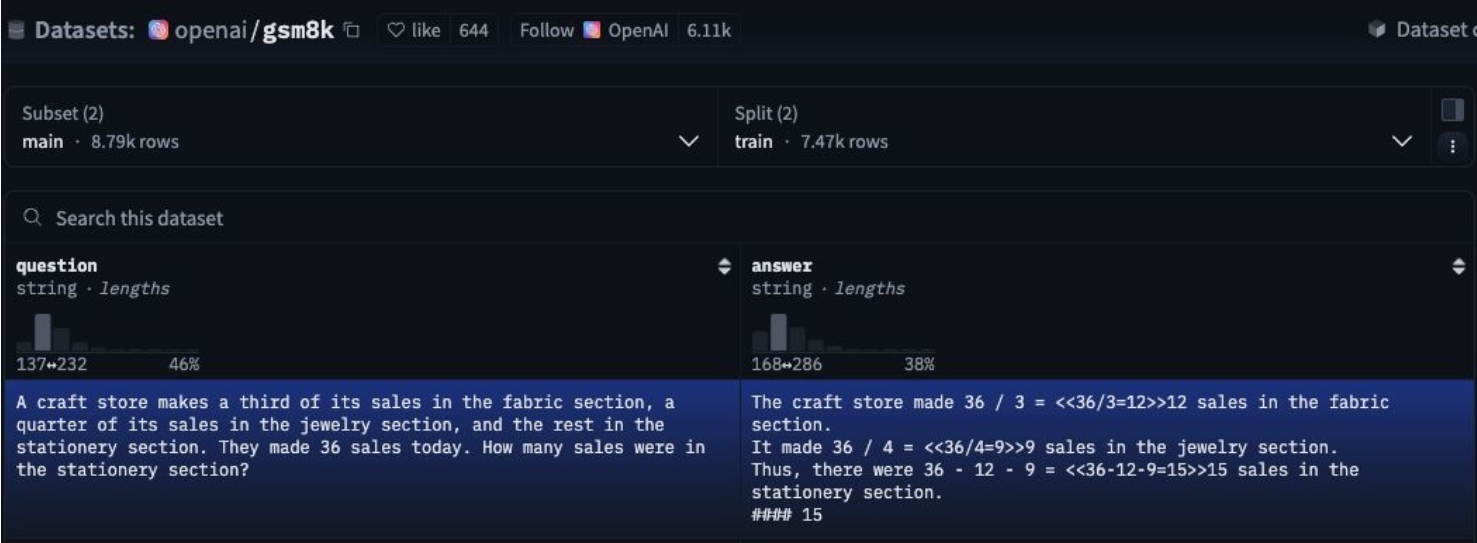
\includegraphics[width=0.9\textwidth]{GSM8k.png} % Replace with your image file
        \caption{Example problem and step-by-step solution from the GSM8K dataset.}
        \label{fig:gsm8k_example}
    \end{figure}

    \item \textbf{MATH dataset \cite{hendrycksmath2021} and MATH 500 subset:}
    Compiled by Hendrycks et al. (2021), the full MATH dataset presents a significant challenge with 12,500 problems from high school mathematics competitions (AMC 10/12, AIME) covering diverse topics like Algebra, Geometry, Number Theory, etc. Problems require deep mathematical understanding and often involve complex symbolic manipulation in LaTeX format. While comprehensive, the scale and difficulty of the full MATH dataset pose significant computational demands for evaluation and iterative fine-tuning, especially when working with SLMs and limited resources.

    Therefore, for more focused evaluation and efficient experimentation within this project, we primarily utilized the \textbf{MATH 500} dataset. This is a commonly used 500-problem subset of the MATH test set, curated to maintain the topic diversity and difficulty range of the original while being significantly more manageable. Using MATH 500 allowed for faster evaluation cycles and provided a representative assessment of model performance on challenging high school math problems without the extensive computational cost of the full dataset. This subset serves to test the upper limits of our models' reasoning abilities on complex, formal mathematical tasks, complementing GSM8K.

    % Placeholder for TWO MATH dataset images (Directory structure + Question)
    \begin{figure}[h!]
        \centering

        % First image: Directory structure
        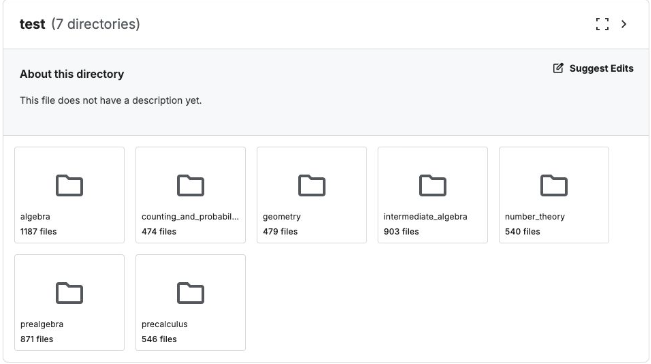
\includegraphics[width=0.7\textwidth]{math1.png} % Replace with your DIRECTORY structure image file

        \vspace{1em} % Add some vertical space between images (adjust '1em' as needed)

        % Second image: Example question
        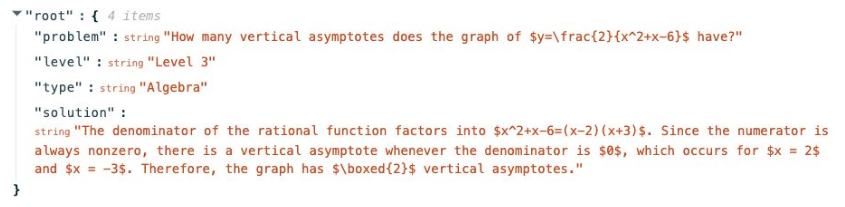
\includegraphics[width=0.9\textwidth]{math2.png} % Replace with your EXAMPLE question image file

        \caption{MATH dataset structure and content example. (Top) Typical directory organization by subject area. (Bottom) An example problem representative of the content within these directories (subset MATH 500).}
        \label{fig:math_structure_example} % Use a label that reflects both images
    \end{figure}


\end{itemize}


Together, GSM8K and MATH provide a comprehensive evaluation suite, assessing both fundamental step-by-step arithmetic reasoning and advanced problem-solving across various mathematical domains.

\subsection{Preprocessing}
To prepare the datasets for model evaluation and fine-tuning, several preprocessing steps were undertaken to structure the data and reliably extract ground truth answers:

\begin{itemize}
    \item \textbf{Regex-based Answer Extraction (GSM8K):}
    For the GSM8K dataset, the final numerical answers are consistently formatted within the provided solutions, typically marked by \#\#\#\#  We implemented a simple regular expression (regex) pattern to automatically parse these solutions and reliably extract the definitive ground truth numerical answer for each problem. This automated approach ensured high accuracy in obtaining the target answers for evaluation against model outputs.

    \item \textbf{Preprocessing Pipeline for MATH dataset:}
    The MATH dataset required a more involved preprocessing pipeline due to its structure and the complexity of its solutions:
    \begin{enumerate}
        \item \textit{Concept-based Organization:} We first processed the dataset by extracting questions from their concept-wise directory structure (e.g., Algebra, Geometry) and organizing them into a structured format, such as a CSV file, associating each question with its corresponding solution and topic.
        \item \textit{Difficulty Filtering:} To focus our evaluation and fine-tuning efforts on sufficiently challenging problems, we filtered the extracted questions, retaining only those designated as difficulty level 4 and level 5, which represent harder high school competition problems.
        \item \textit{Zero-shot Gemini 2.0 for Ground Truth Estimation:} Unlike GSM8K's simple final answer format, MATH solutions are often complex derivations in LaTeX. Manually extracting the final answer from thousands of such solutions is time-consuming and error-prone. To obtain a standardized ground truth answer for evaluation, we employed Google's Gemini-2.0-Flash model in a zero-shot prompting setup. We provided the model with the problem statement and the full LaTeX solution, asking it to identify and extract the final answer. While not infallible, this provided a scalable method for estimating ground truth answers from complex solution texts.
        \item \textit{Final Dataset Curation:} After these steps, our processed MATH subset consisted of 2538 questions suitable for our experiments. The original detailed LaTeX solutions were retained alongside the extracted answers for potential future analysis or comparison of reasoning steps.
    \end{enumerate}

\end{itemize}
These preprocessing steps were crucial for creating standardized evaluation sets and ensuring that model performance could be measured accurately and efficiently against reliable ground truth answers extracted from the diverse formats of the source datasets.


\section{Experiments and Results}
\subsection{Baseline Performance}
Before applying fine-tuning techniques like GRPO, we established the baseline mathematical reasoning performance of our selected models. These evaluations were conducted using zero-shot or few-shot prompting on the preprocessed GSM8K and MATH 500 datasets. The goal was to understand the initial capabilities of each model, quantify the advantage of domain-specific pre-training (Qwen2.5-MATH vs. Qwen2-1.5B), and establish reference points for measuring improvement. The results also allow comparison against a high-performance public model (Gemini-2.0-Flash).

Table \ref{tab:baseline_performance} summarizes the baseline accuracy achieved by each model. The 'Role' column clarifies whether the model served as a primary target for fine-tuning within SPARK or was included mainly for comparison purposes.

\begin{table}[htbp] % Use [htbp] for better float placement
\centering
\caption{Baseline model performance on GSM8K and MATH 500 datasets, indicating model roles.}
\label{tab:baseline_performance}
\begin{tabular}{@{}l c c l@{}} % Use booktabs style: l=left, c=center. @{} removes extra space.
\toprule
\textbf{Model} & \textbf{GSM8K Acc.} & \textbf{MATH 500 Acc.} & \textbf{Role} \\
\midrule
Qwen2-1.5B-Instruct & 59.82\% & 19.23\% & Comparison Baseline \\
Qwen2.5-MATH-1.5B (4-bit) & 76.80\% & 24.43\% & Main Model (Target) \\
Phi-mini-4k-instruct (4-bit) & 78.04\% & 18.85\% & Main Model (Target) \\ % <-- ADD YOUR PHI-MINI RESULTS HERE
Gemini-2.0-Flash & 72.78\% & 33.69\% & High-Perf. Benchmark \\
\bottomrule
\end{tabular}
\end{table}

Initial observations from the baseline results indicate that the domain-specific Qwen2.5-MATH model significantly outperforms its generalist counterpart (Qwen2-1.5B) on both datasets, validating the benefit of math-focused pre-training. While the SLMs show promising capability, especially Qwen2.5-MATH on GSM8K, they lag behind the larger Gemini model, particularly on the more complex MATH 500 problems. This highlights the challenge and the opportunity for improvement through targeted fine-tuning.

\begin{figure}
    \centering
    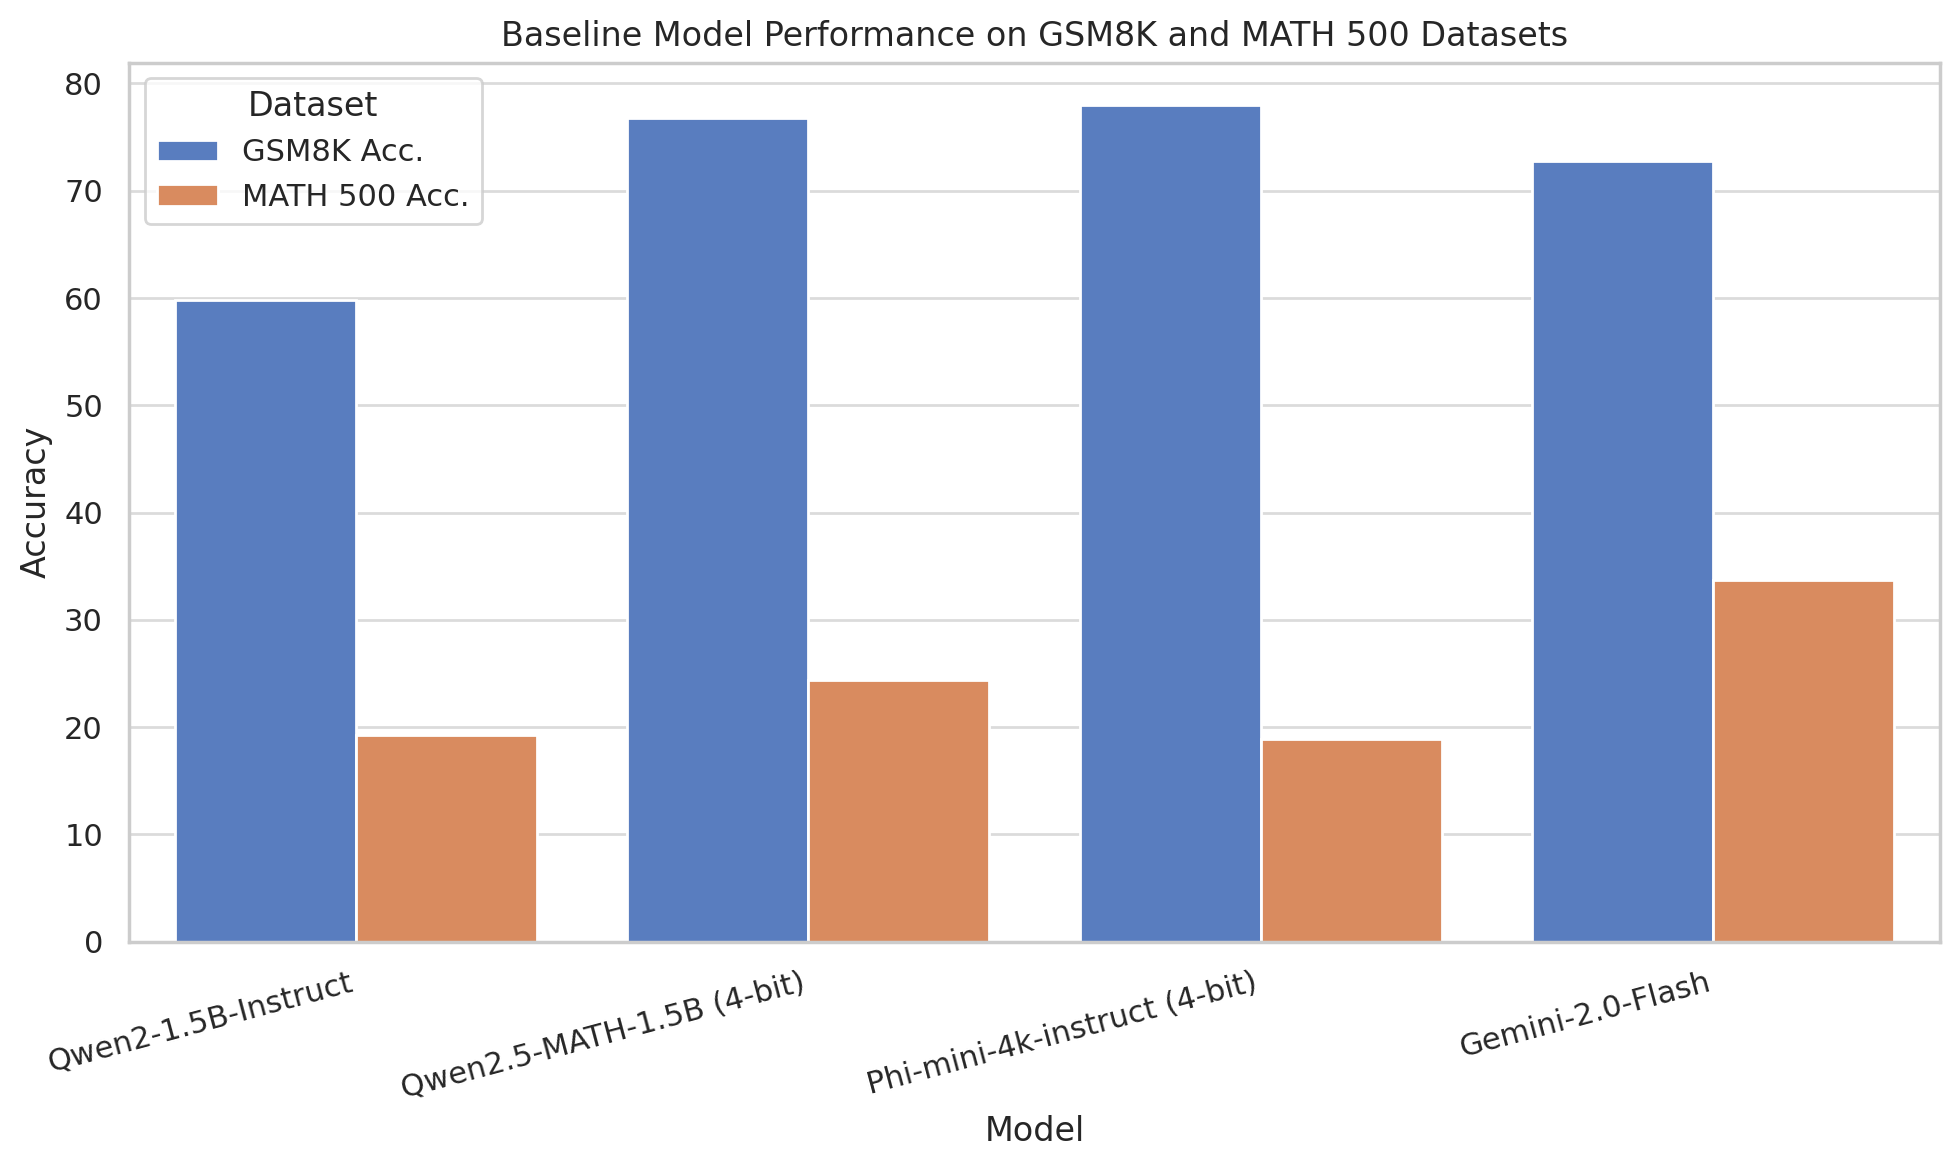
\includegraphics[width=1\linewidth]{Baseline result.png}
    \caption{Results of Baseline}
    \label{fig:enter-label}
\end{figure}



\subsection{Post-Hoc Error Analysis}
Beyond the aggregate accuracy scores from the baseline evaluations, a qualitative post-hoc analysis was conducted on the model outputs to understand the nature of the errors. This involved manually inspecting incorrect or incomplete solutions generated by the models, particularly Qwen2.5-MATH and Phi-mini, on both GSM8K and MATH 500. Several recurring patterns emerged:

\begin{itemize}
    \item \textbf{Inconsistent Output Formatting:} A significant challenge, especially noticeable with the smaller Qwen models, was the lack of strict adherence to a consistent format for numerical answers. While evaluation scripts often expect a precise format (e.g., `6600`), models might produce variations like comma-separated numbers (`6,600`), floating-point representations (`6600.0`), or even fractional forms (`6600/1`). This inconsistency, while sometimes numerically equivalent, complicates automated answer verification and necessitates robust parsing logic or fine-tuning for format compliance.

    % % Placeholder for Formatting Issue Image
    % \begin{figure}[h!]
    %     \centering
    %     \includegraphics[width=0.8\textwidth]{placeholder.png} % Replace with your image file
    %     \caption{Examples of inconsistent numerical answer formatting observed in model outputs compared to the expected format.}
    %     \label{fig:format_issue}
    % \end{figure}

    \item \textbf{Incomplete Solutions and Early Stopping:} Models frequently failed to complete the entire reasoning process, stopping prematurely. This often manifested as partially correct solutions that lacked the final steps to reach the answer. Such errors could sometimes be attributed to inherent output length limitations of the models or contexts, but other times suggested a breakdown in the reasoning chain. Analyzing whether the initial steps were "directionally correct" was crucial here; cases where the approach was sound but stopped early might be fixable with prompting strategies encouraging longer generation or increased length limits, whereas abrupt stops mid-calculation often pointed to deeper issues.

    % Placeholder for Incomplete Solution Image
    \begin{figure}[h!]
        \centering
        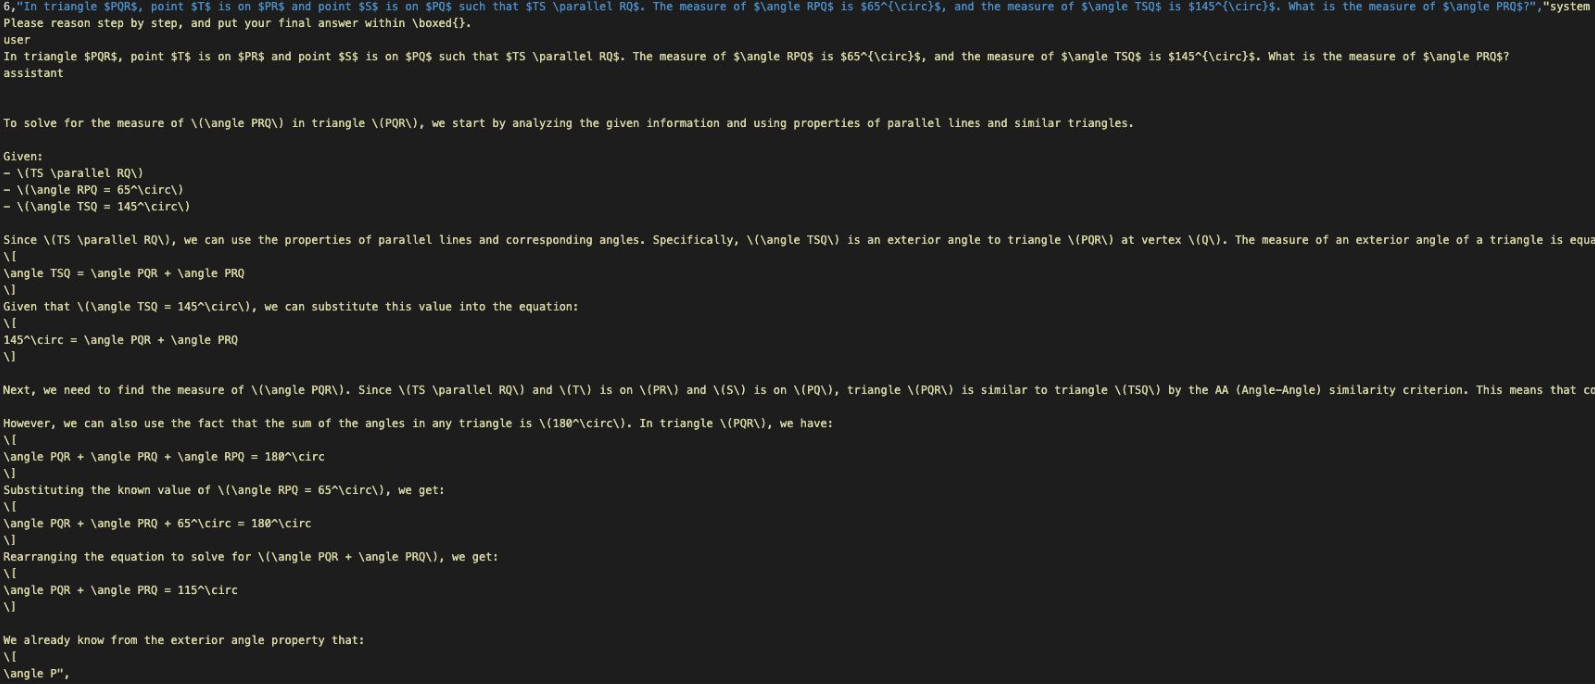
\includegraphics[width=0.9\textwidth]{incomplete.png} % Replace with your image file
        \caption{An example of a model output showing a partially correct reasoning chain that stops before reaching the final answer.}
        \label{fig:incomplete_sol}
    \end{figure}

    \item \textbf{Flawed Reasoning and Conceptual Gaps:} This category encompasses errors stemming from fundamental misunderstandings or incorrect application of mathematical principles. We observed two key sub-types:
        \begin{itemize}
            \item \textit{Incorrect Approach from Start:} In some cases, the model initiated the solution with an entirely wrong strategy or misinterpreted the problem's core requirements, indicating a fundamental gap in understanding or planning.
            \item \textit{Conceptual Knowledge Deficits:} Particularly evident in the challenging MATH dataset problems, models sometimes lacked the necessary specific knowledge (e.g., advanced algebraic manipulations, geometric theorems, number theory concepts) required to proceed correctly, even if the overall structure of the problem was grasped. This often led to incorrect intermediate steps or the inability to navigate complex proofs.
        \end{itemize}
    These errors highlight the limitations in the models' underlying mathematical knowledge base and procedural reasoning capabilities, representing core challenges that fine-tuning aims to address. Loss of logical coherence in longer multi-step solutions was also a common failure mode within this category.

    % Placeholder for Reasoning Error Image
    % \begin{figure}[h!]
    %     \centering
    %     \includegraphics[width=0.9\textwidth]{placeholder_reasoning_error.png} % Replace with your image file
    %     \caption{Illustration of a flawed reasoning step or a conceptual error observed in a model's solution attempt.}
    %     \label{fig:reasoning_error}
    % \end{figure}

\end{itemize}
Understanding these distinct error types provided valuable insights for guiding the fine-tuning process, particularly for designing preference data for methods like GRPO, where rewarding outputs that avoid these pitfalls (e.g., correctly formatted, complete, logically sound) is essential.

\subsection{RL-based Fine-Tuning (GRPO)}

To address the shortcomings identified during the baseline evaluation and error analysis, we employed Group Relative Policy Optimization (GRPO) for fine-tuning our primary SLMs. GRPO is a preference-based reinforcement learning technique that offers a computationally efficient alternative to traditional methods like PPO with a learned reward model. It operates by sampling multiple candidate responses from the current policy for a given prompt, grouping these responses, and identifying the relatively "best" response within that group based on defined preference criteria. The policy is then updated directly to increase the probability of generating outputs similar to the preferred ones, effectively steering the model towards desired behaviors without needing an explicit reward score for every response. This approach is particularly well-suited for optimizing SLMs on consumer-grade hardware.

% Placeholder for GRPO Process Image
% \begin{figure}[h!]
%     \centering
%     \includegraphics[width=0.8\textwidth]{placeholder_grpo_process.png} % Replace with your GRPO illustration
%     \caption{Conceptual overview of the Group Relative Policy Optimization (GRPO) feedback loop used for fine-tuning.}
%     \label{fig:grpo_process}
% \end{figure}

We applied GRPO fine-tuning specifically to our target SLMs:

\begin{itemize}
    \item \textbf{Fine-tuning Qwen2.5-MATH-1.5B (4-bit):}
    Leveraging the Unsloth library for efficient 4-bit training with LoRA (rank \texttt{r=16}, alpha \texttt{16}), we fine-tuned the Qwen2.5-MATH model using GRPO. Key hyperparameters included a learning rate (\texttt{LEARNING\_RATE}) of \texttt{5e-6}, a group size (\texttt{NUM\_GENERATIONS}) of \texttt{6}, a maximum sequence length (\texttt{MAX\_SEQ\_LENGTH}) of \texttt{786}, gradient accumulation over \texttt{8} steps (effective batch size 8), and training for \texttt{6000} steps.

    The preference criteria for GRPO were implemented as a combination of Python reward functions, specifically targeting the baseline issues of correctness, completeness, and formatting, with a focus on the model's native \verb|\boxed{}| answer format:

        \begin{itemize}
            \item \textit{Correctness Reward (\texttt{correctness\_reward\_func}):} This function directly addressed accuracy by extracting the content within the \verb|\boxed{}| block from each generated response and comparing it to the ground truth answer. A significant reward (\texttt{2.0}) was assigned for an exact match, incentivizing the model to produce the correct final result. Responses where the answer couldn't be extracted or matched received zero reward.

\begin{lstlisting}[language=Python, caption={Core logic for correctness reward (Qwen)}, label={lst:qwen_correct}]
def correctness_reward_func(...):
    # ... extract responses ...
    extracted_responses = [extract_boxed_answer(r) for r in responses]
    # ... compare extracted_responses to correct_answers ...
    if extracted == corr_ans:
        rewards.append(2.0)
    else:
        rewards.append(0.0)
    return rewards
\end{lstlisting}


            \item \textit{Integer Format Reward (\texttt{int\_reward\_func}):} To encourage consistent formatting for numerical answers, particularly integers (common in GSM8K), this function provided a small positive reward (\texttt{0.5}) if the content extracted from the \verb|\boxed{}| block consisted only of digits. This subtly guides the model towards cleaner numerical outputs.
\begin{lstlisting}[language=Python, caption={Core logic for correctness reward (Qwen)}, label={lst:qwen_correct}]
def int_reward_func(...):
    # ... extract response ...
    extracted_response = extract_boxed_answer(response)
    # Provide 0.5 reward if extracted answer is purely digits
    batch_rewards.append(0.5 if extracted_response.isdigit() else 0.0)
    return rewards
\end{lstlisting}

            \item \textit{Overall Length Reward (\texttt{length\_reward\_func}):} To counteract premature stopping and encourage more detailed solutions, this function rewarded longer overall completions. The length was estimated by a simple token counting heuristic (\texttt{count\_tokens\_hardcoded}) and normalized relative to \texttt{MAX\_SEQ\_LENGTH}. The reward was scaled (\texttt{0.5}) to avoid dominating other criteria.
\begin{lstlisting}[language=Python, caption={Core logic for Overall Length reward (Qwen)}, label={lst:qwen_correct}]
def length_reward_func(...):
    # ... get response ...
    length = count_tokens_hardcoded(response)
    # Normalize length and scale reward
    normalized_length = min(length / MAX_SEQ_LENGTH, 1.0)
    reward = 0.5 * normalized_length
    batch_rewards.append(reward)
    return rewards
\end{lstlisting}

            \item \textit{Reasoning Length Reward (\texttt{reasoning\_length\_reward\_func}):} Distinct from overall length, this specifically rewarded the length of the reasoning *before* the final \verb|\boxed{}| answer. This incentivizes the generation of more thorough step-by-step derivations, addressing the need for interpretability and logical coherence identified in the error analysis. The length was again estimated, normalized (relative to 80% of \texttt{MAX\_SEQ\_LENGTH}), and scaled (\texttt{0.5}).
\begin{lstlisting}[language=Python, caption={Core logic for Reasoning Length Reward (Qwen)}, label={lst:qwen_correct}]
def reasoning_length_reward_func(...):
    # ... get response ...
    boxed_match = re.search(r"\\boxed\{", response)
    if boxed_match:
        reasoning_part = response[:boxed_match.start()]
    else:
        reasoning_part = response # Consider full response if no box
    length = count_tokens_hardcoded(reasoning_part)
    normalized_length = min(length / (MAX_SEQ_LENGTH * 0.8), 1.0)
    reward = 0.5 * normalized_length
    batch_rewards.append(reward)
    return rewards
\end{lstlisting}
        \end{itemize}
    The combination of these reward functions aimed to guide the Qwen model towards generating solutions that are not only correct but also complete, well-formatted, and demonstrate clear reasoning steps.

    \begin{itemize}
    
    \item \textbf{Fine-tuning Phi-mini-4k-instruct (4-bit):}
    GRPO was applied to the \texttt{unsloth/Phi-4-mini-instruct} model using Unsloth and LoRA (\texttt{r=8}). Training configuration included \texttt{MAX\_SEQ\_LENGTH=768}, LR \texttt{5e-6}, \texttt{NUM\_GENERATIONS=2} (completions per prompt), gradient accumulation \texttt{1}, and \texttt{16000} steps. A key difference was guiding Phi-mini towards a structured XML format via a system prompt and tailored reward functions:
    \begin{itemize}
        \item \textit{Correctness Reward (\texttt{correctness\_reward\_func}):} Assigned reward \texttt{2.0} for correctness. This used a robust extraction function (\texttt{extract\_xml\_answer}) attempting to find the answer first within LaTeX \verb|\boxed{}|, then within XML \verb|<answer>...</answer>| tags, and finally falling back to the last number sequence in the completion if neither tag was found. A reward of \texttt{2.0} was given for exact matches against the ground truth answer, and \texttt{0.0} otherwise.
        \begin{lstlisting}[language=Python, caption={Robust answer extraction logic for Phi correctness}, label={lst:phi_extract_updated}]
        def extract_xml_answer(text: str) -> str:
            # Try to extract from LaTeX boxed format first
            latex_match = re.search(r"\\boxed\{([\d\.]+)\}", text)
            if latex_match:
                extracted = latex_match.group(1)
            else:
                # If LaTeX extraction fails, extract from XML <answer> tags
                answer_match = re.search(r"<answer>\s*(.*?)\s*</answer>", text, re.DOTALL)
                extracted = answer_match.group(1).strip() if answer_match else None
            # If nothing was found, try to extract the last number as a fallback
            if extracted is None:
                number_match = re.search(r"(\d+\.?\d*)$", text)
                extracted = number_match.group(1) if number_match else None
            return extracted if extracted is not None else "N/A"
        \end{lstlisting}
        

        \item \textit{Overall Length Reward (\texttt{length\_reward\_func}):} Counteracted premature stopping by rewarding longer overall completions. Length was estimated using a simple heuristic (\texttt{count\_tokens\_hardcoded}), normalized relative to \texttt{MAX\_SEQ\_LENGTH} (capped at 1.0), and scaled by \texttt{0.5}.
        \begin{lstlisting}[language=Python, caption={Overall length reward logic (Phi)}, label={lst:phi_len}]
        def length_reward_func(completions: List[List[Dict[str, str]]], **kwargs):
            # ... iterate through completions ...
            length = count_tokens_hardcoded(response)
            # Normalize length and scale reward
            normalized_length = min(length / MAX_SEQ_LENGTH, 1.0)
            reward = 0.5 * normalized_length
            batch_rewards.append(reward)
            # ... extend rewards ...
            return rewards
        \end{lstlisting}

        
        \item \textit{Reasoning Length Reward (\texttt{reasoning\_length\_reward\_func}):} Specifically rewarded the length of the reasoning *before* the final \verb|\boxed{}| answer marker (note: it searches for LaTeX \verb|\boxed{| specifically, not the XML `<answer>` tag, to delimit reasoning). The length was estimated (\texttt{count\_tokens\_hardcoded}), normalized relative to 80% of \texttt{MAX\_SEQ\_LENGTH} (capped at 1.0), and scaled by \texttt{0.5}.
        \begin{lstlisting}[language=Python, caption={Reasoning length reward logic (Phi)}, label={lst:phi_reasonlen}]
        def reasoning_length_reward_func(completions: List[List[Dict[str, str]]], **kwargs):
            # ... iterate through completions ...
            boxed_match = re.search(r"\\boxed\{", response) # Looks for LaTeX box start
            if boxed_match:
                reasoning_part = response[:boxed_match.start()]
            else:
                reasoning_part = response # Consider full response if no box
            length = count_tokens_hardcoded(reasoning_part)
            # Normalize vs 80% of max length and scale reward
            normalized_length = min(length / (MAX_SEQ_LENGTH * 0.8), 1.0)
            reward = 0.5 * normalized_length
            batch_rewards.append(reward)
            # ... extend rewards ...
            return rewards
        \end{lstlisting}

        \item \textit{XML Format Adherence Reward (\texttt{xmlcount\_reward\_func}):} Unique to the Phi fine-tuning, this explicitly rewarded the target XML structure. It checked for the exact presence (\texttt{.count(...) == 1}) of key tags including newlines (\verb|<reasoning>\n|, \verb|\n</reasoning>\n|, \verb|\n<answer>\n|, \verb|\n</answer>|) assigning partial rewards (\texttt{0.125} each). It also penalized extraneous text after the final \verb|\n</answer>| tag based on character length.
        \begin{lstlisting}[language=Python, caption={XML structure adherence reward (Phi)}, label={lst:phi_xmlcount_updated}]
        def count_xml(text) -> float:
            count = 0.0
            # Check for exact tag presence with specific newlines
            if text.count("<reasoning>\n") == 1: count += 0.125
            if text.count("\n</reasoning>\n") == 1: count += 0.125
            if text.count("\n<answer>\n") == 1: count += 0.125
            if text.count("\n</answer>") == 1: count += 0.125 # Check for closing tag
        
            # Penalize extra text after closing tag variants
            # (Note: The code checks two slightly different splits for penalty)
            if "\n</answer>\n" in text: # Penalty based on split with two newlines
                 count -= len(text.split("\n</answer>\n")[-1])*0.001
            # Penalty based on split with one newline (catches trailing chars/spaces)
            if "\n</answer>" in text:
                count -= (len(text.split("\n</answer>")[-1]) - 1)*0.001 # -1 for potential final newline
        
            return count
        
        def xmlcount_reward_func(completions, **kwargs) -> list[float]:
            contents = [completion[0]["content"] for completion in completions]
            return [count_xml(c) for c in contents]
        \end{lstlisting}

    \end{itemize}
    The GRPO strategy for Phi-mini thus balanced correctness and completeness with explicit incentives for adopting the desired XML structure, using the specific parameters and reward logic detailed above.
\end{itemize}


By iteratively applying GRPO with preference criteria targeted at common failure modes, the fine-tuning process aimed to enhance the models' abilities to produce more complete and logically coherent answers while also improving formatting consistency, ultimately leading to better performance on the benchmark tasks.


\section{Training Analyses}
\subsection{GRPO Fine-Tuning Analysis: Qwen2.5-MATH}

To understand the impact of GRPO fine-tuning on the Qwen2.5-MATH-1.5B model, we monitored several key metrics during the training process. These metrics provide insights into how the model's behavior evolved under the influence of the combined preference reward functions. The analysis is based on logs visualized over the 6000 training steps (Figure \ref{fig:grpo_qwen_analysis}).

\begin{figure}[htbp]
    \centering
    % First row of images
    \begin{minipage}{0.48\textwidth}
        \centering
        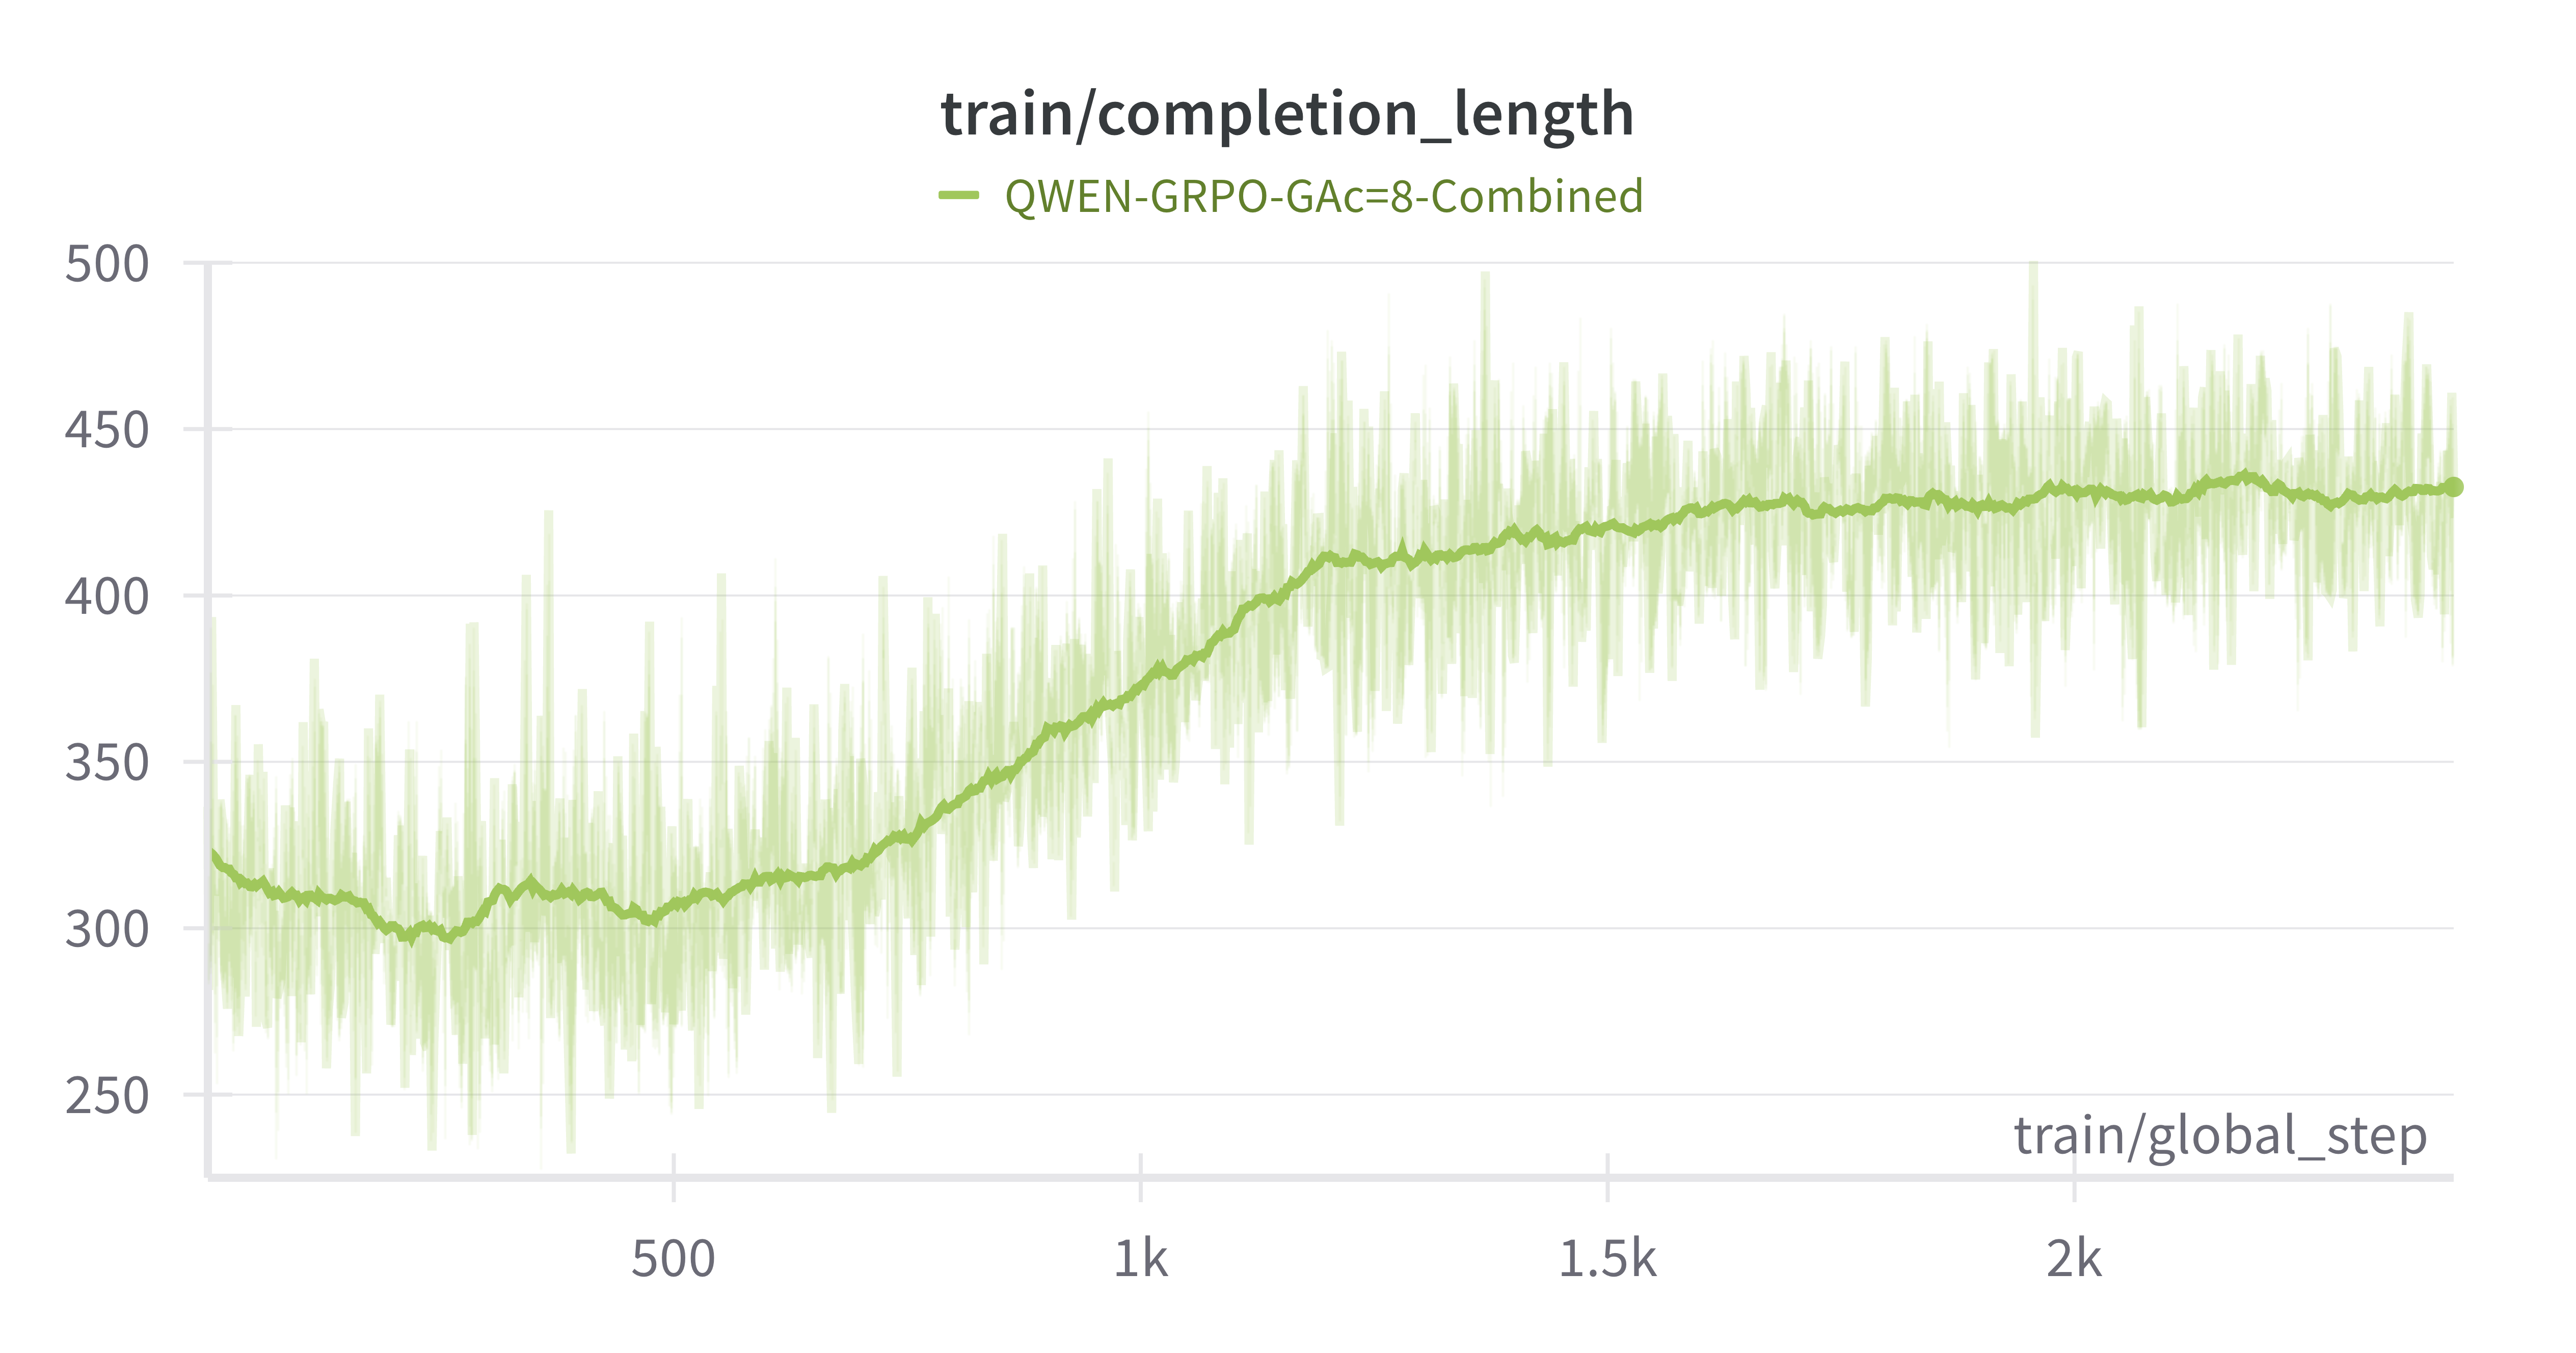
\includegraphics[width=\linewidth]{Qwen/completion_length.png} % Replace with your actual image file
        \caption*{(a) Completion Length} % Unnumbered caption for subfigure
        %\label{fig:qwen_len_graph} % Optional sub-label
    \end{minipage}\hfill % Pushes the minipages apart
    \begin{minipage}{0.48\textwidth}
        \centering
        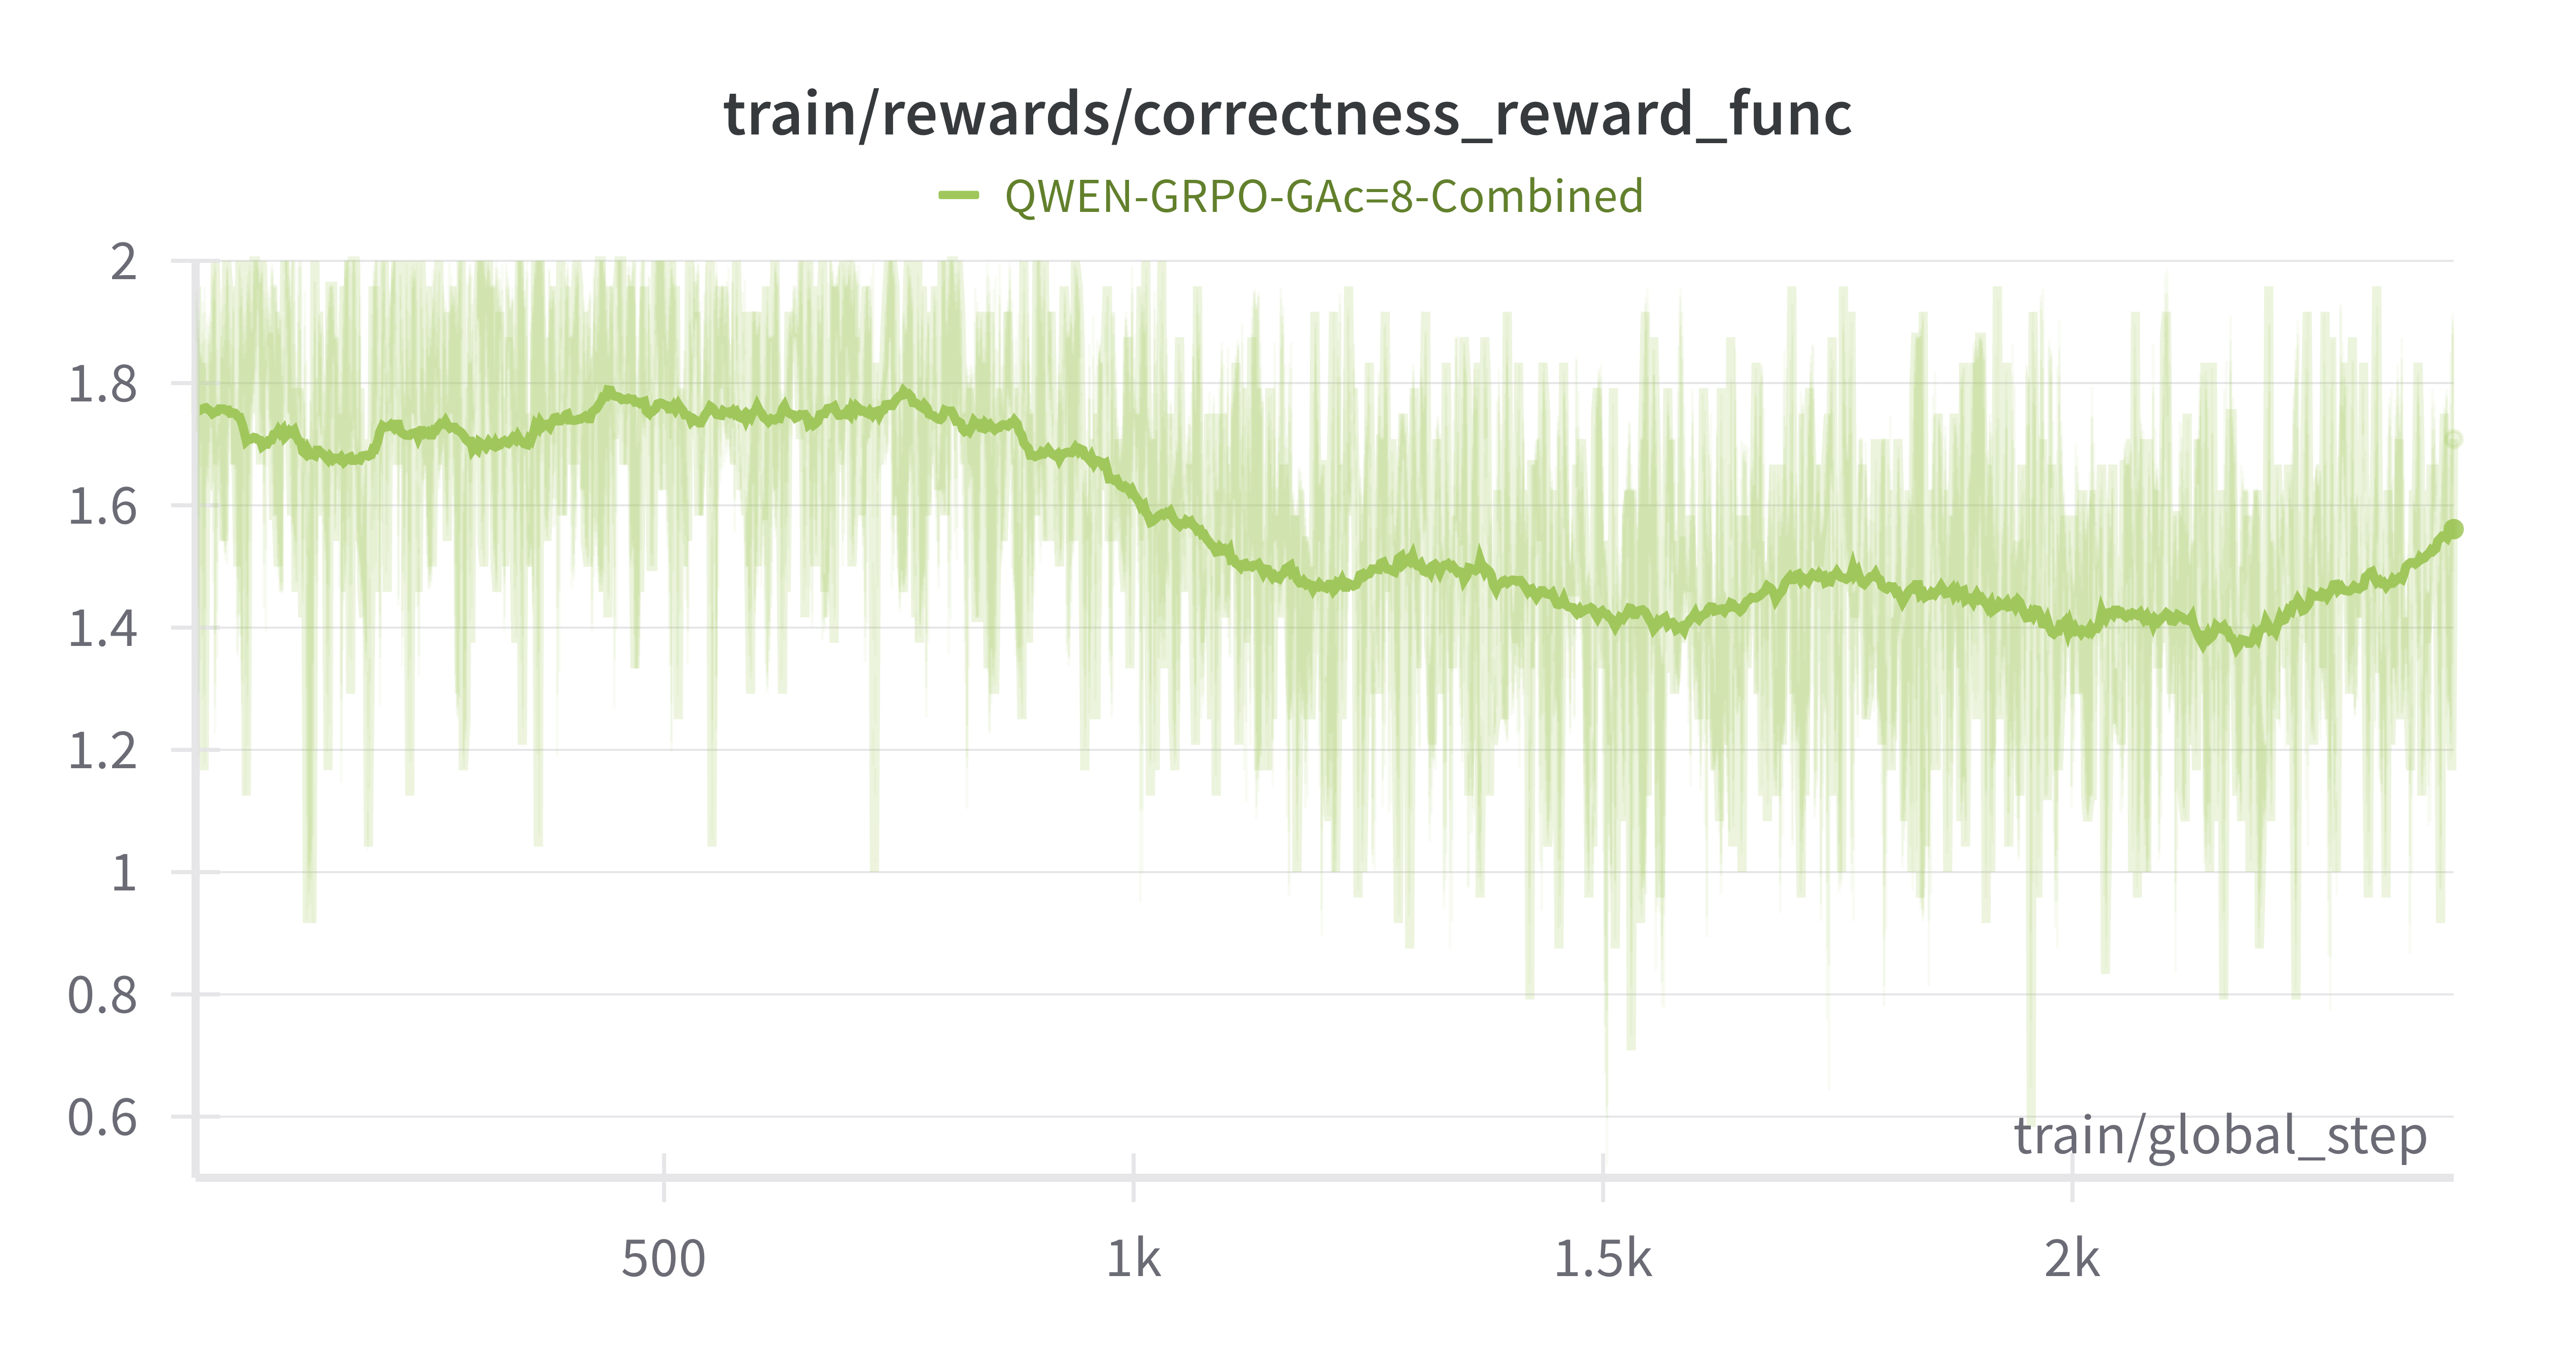
\includegraphics[width=\linewidth]{Qwen/corr_reward.png} % Replace with your actual image file
        \caption*{(b) Correctness Reward}
        %\label{fig:qwen_correct_graph} % Optional sub-label
    \end{minipage}

    \vspace{1em} % Add some vertical space between rows

    % Second row of images
    \begin{minipage}{0.48\textwidth}
        \centering
        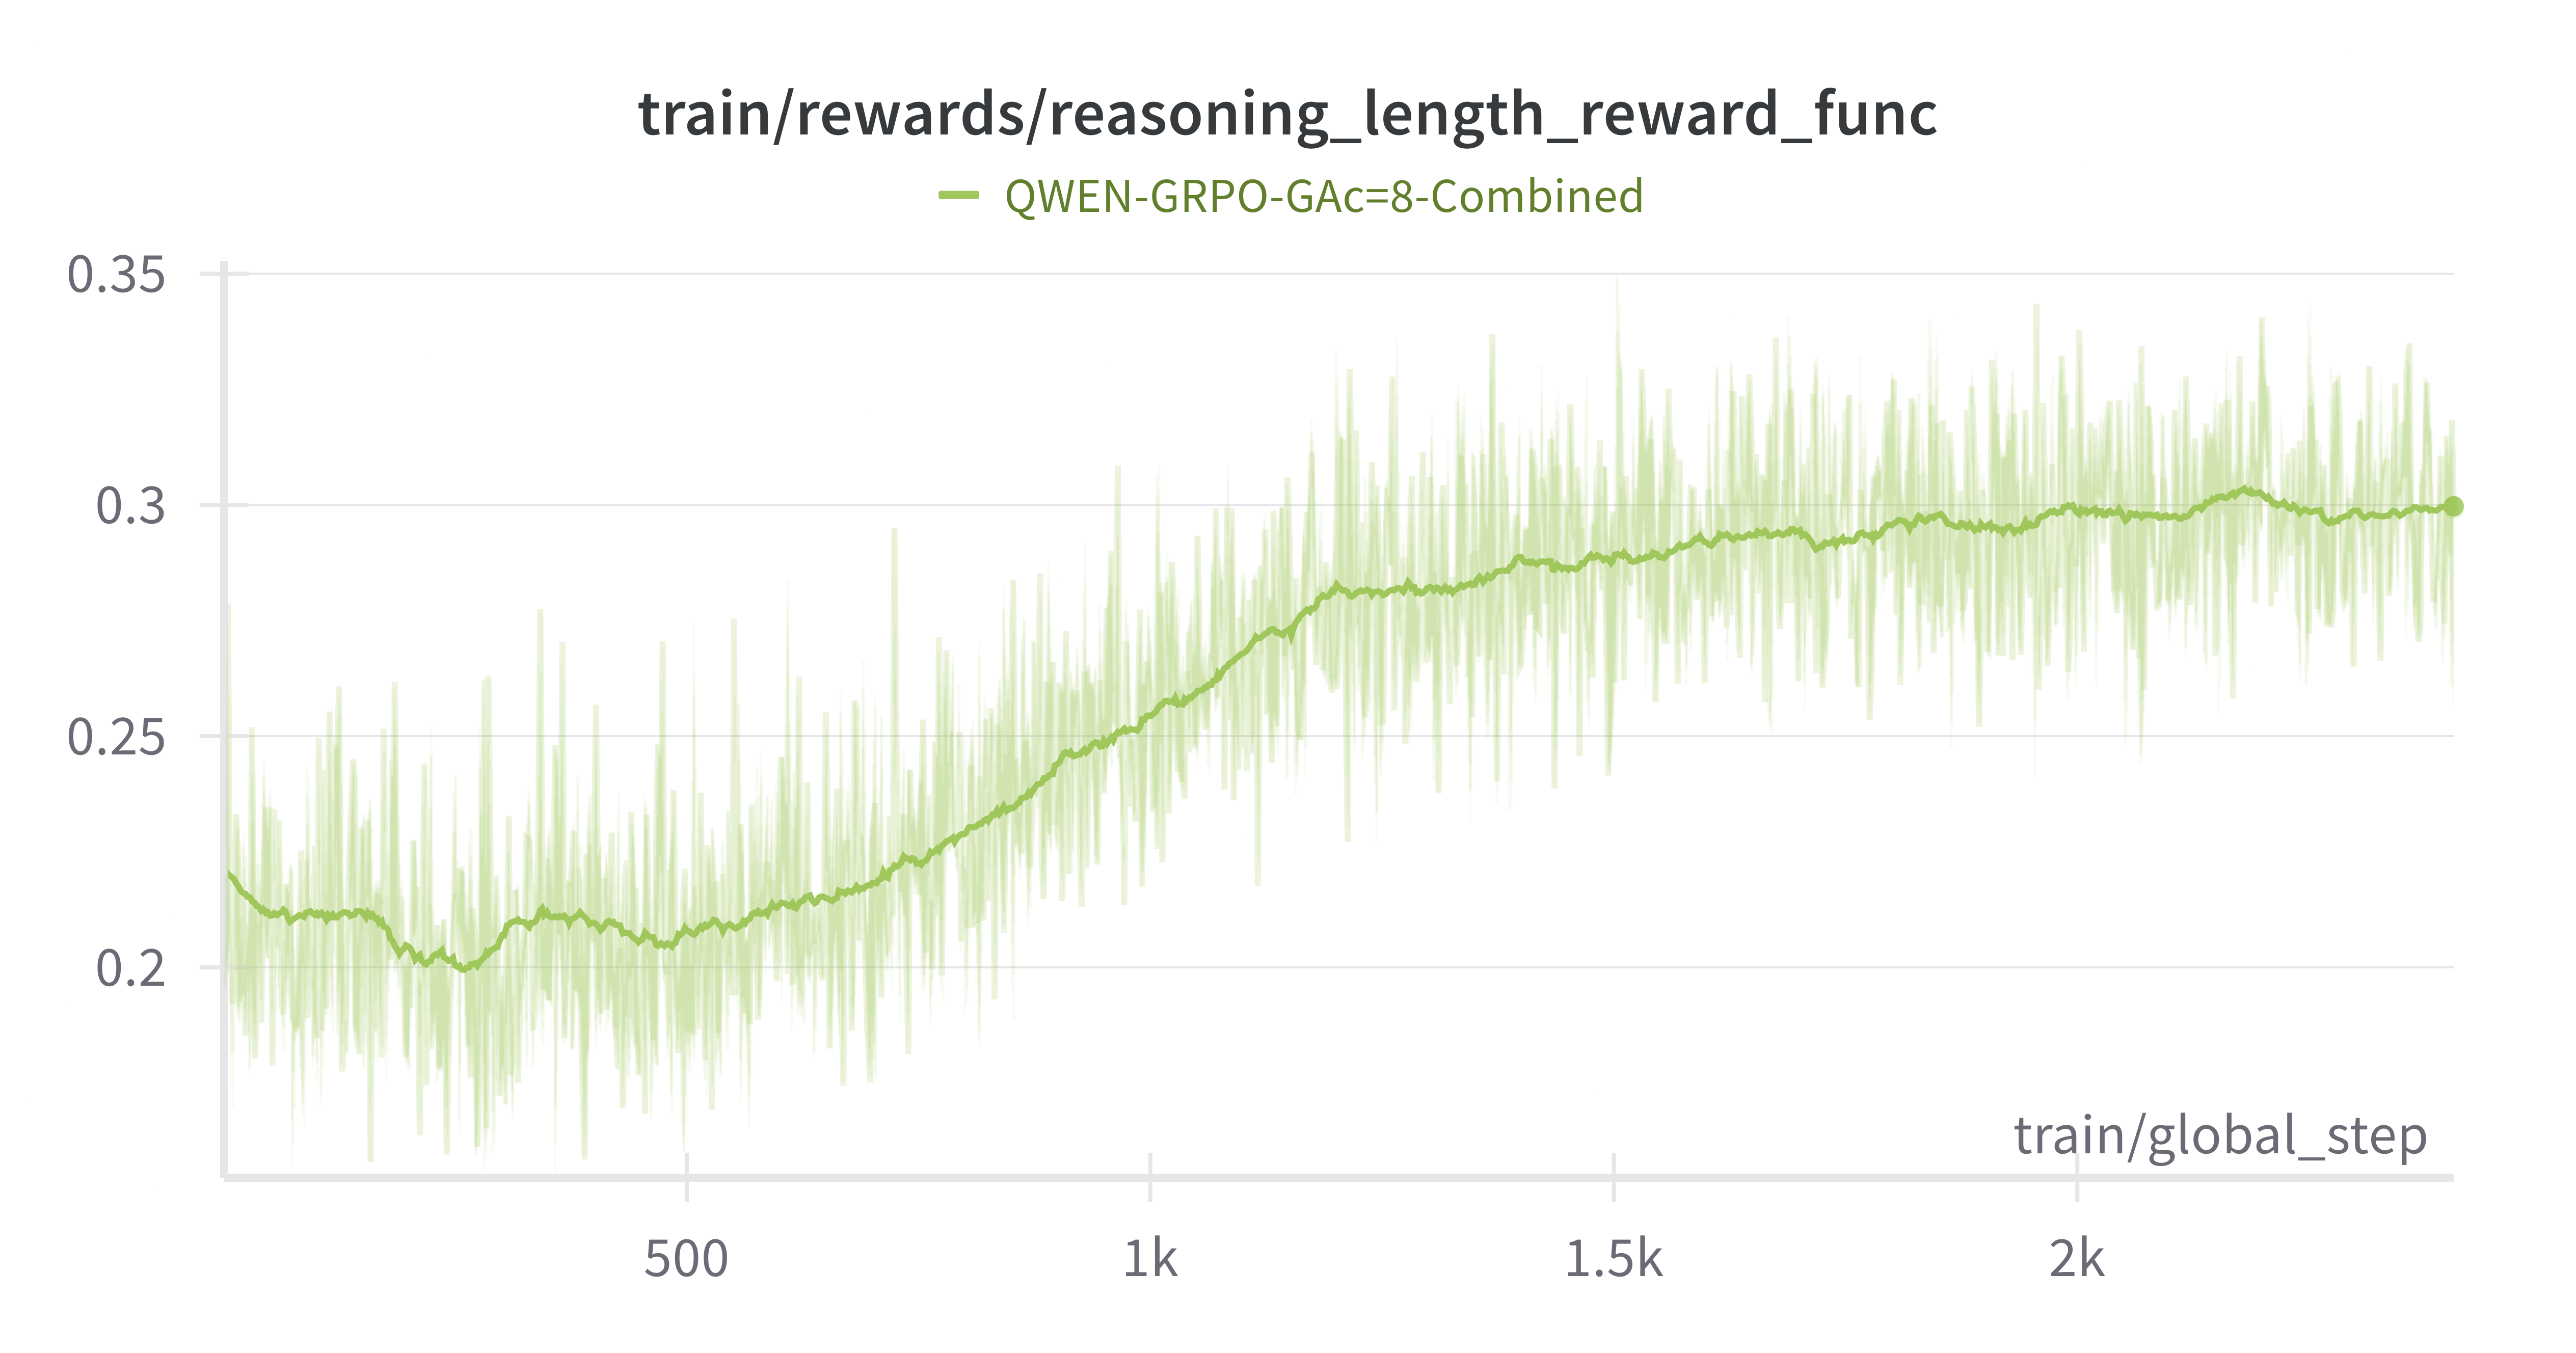
\includegraphics[width=\linewidth]{Qwen/reasoning_length_reward.png} % Replace with your actual image file
        \caption*{(c) Reasoning Length}
        %\label{fig:qwen_reasonlen_graph} % Optional sub-label
    \end{minipage}\hfill
    \begin{minipage}{0.48\textwidth}
        \centering
        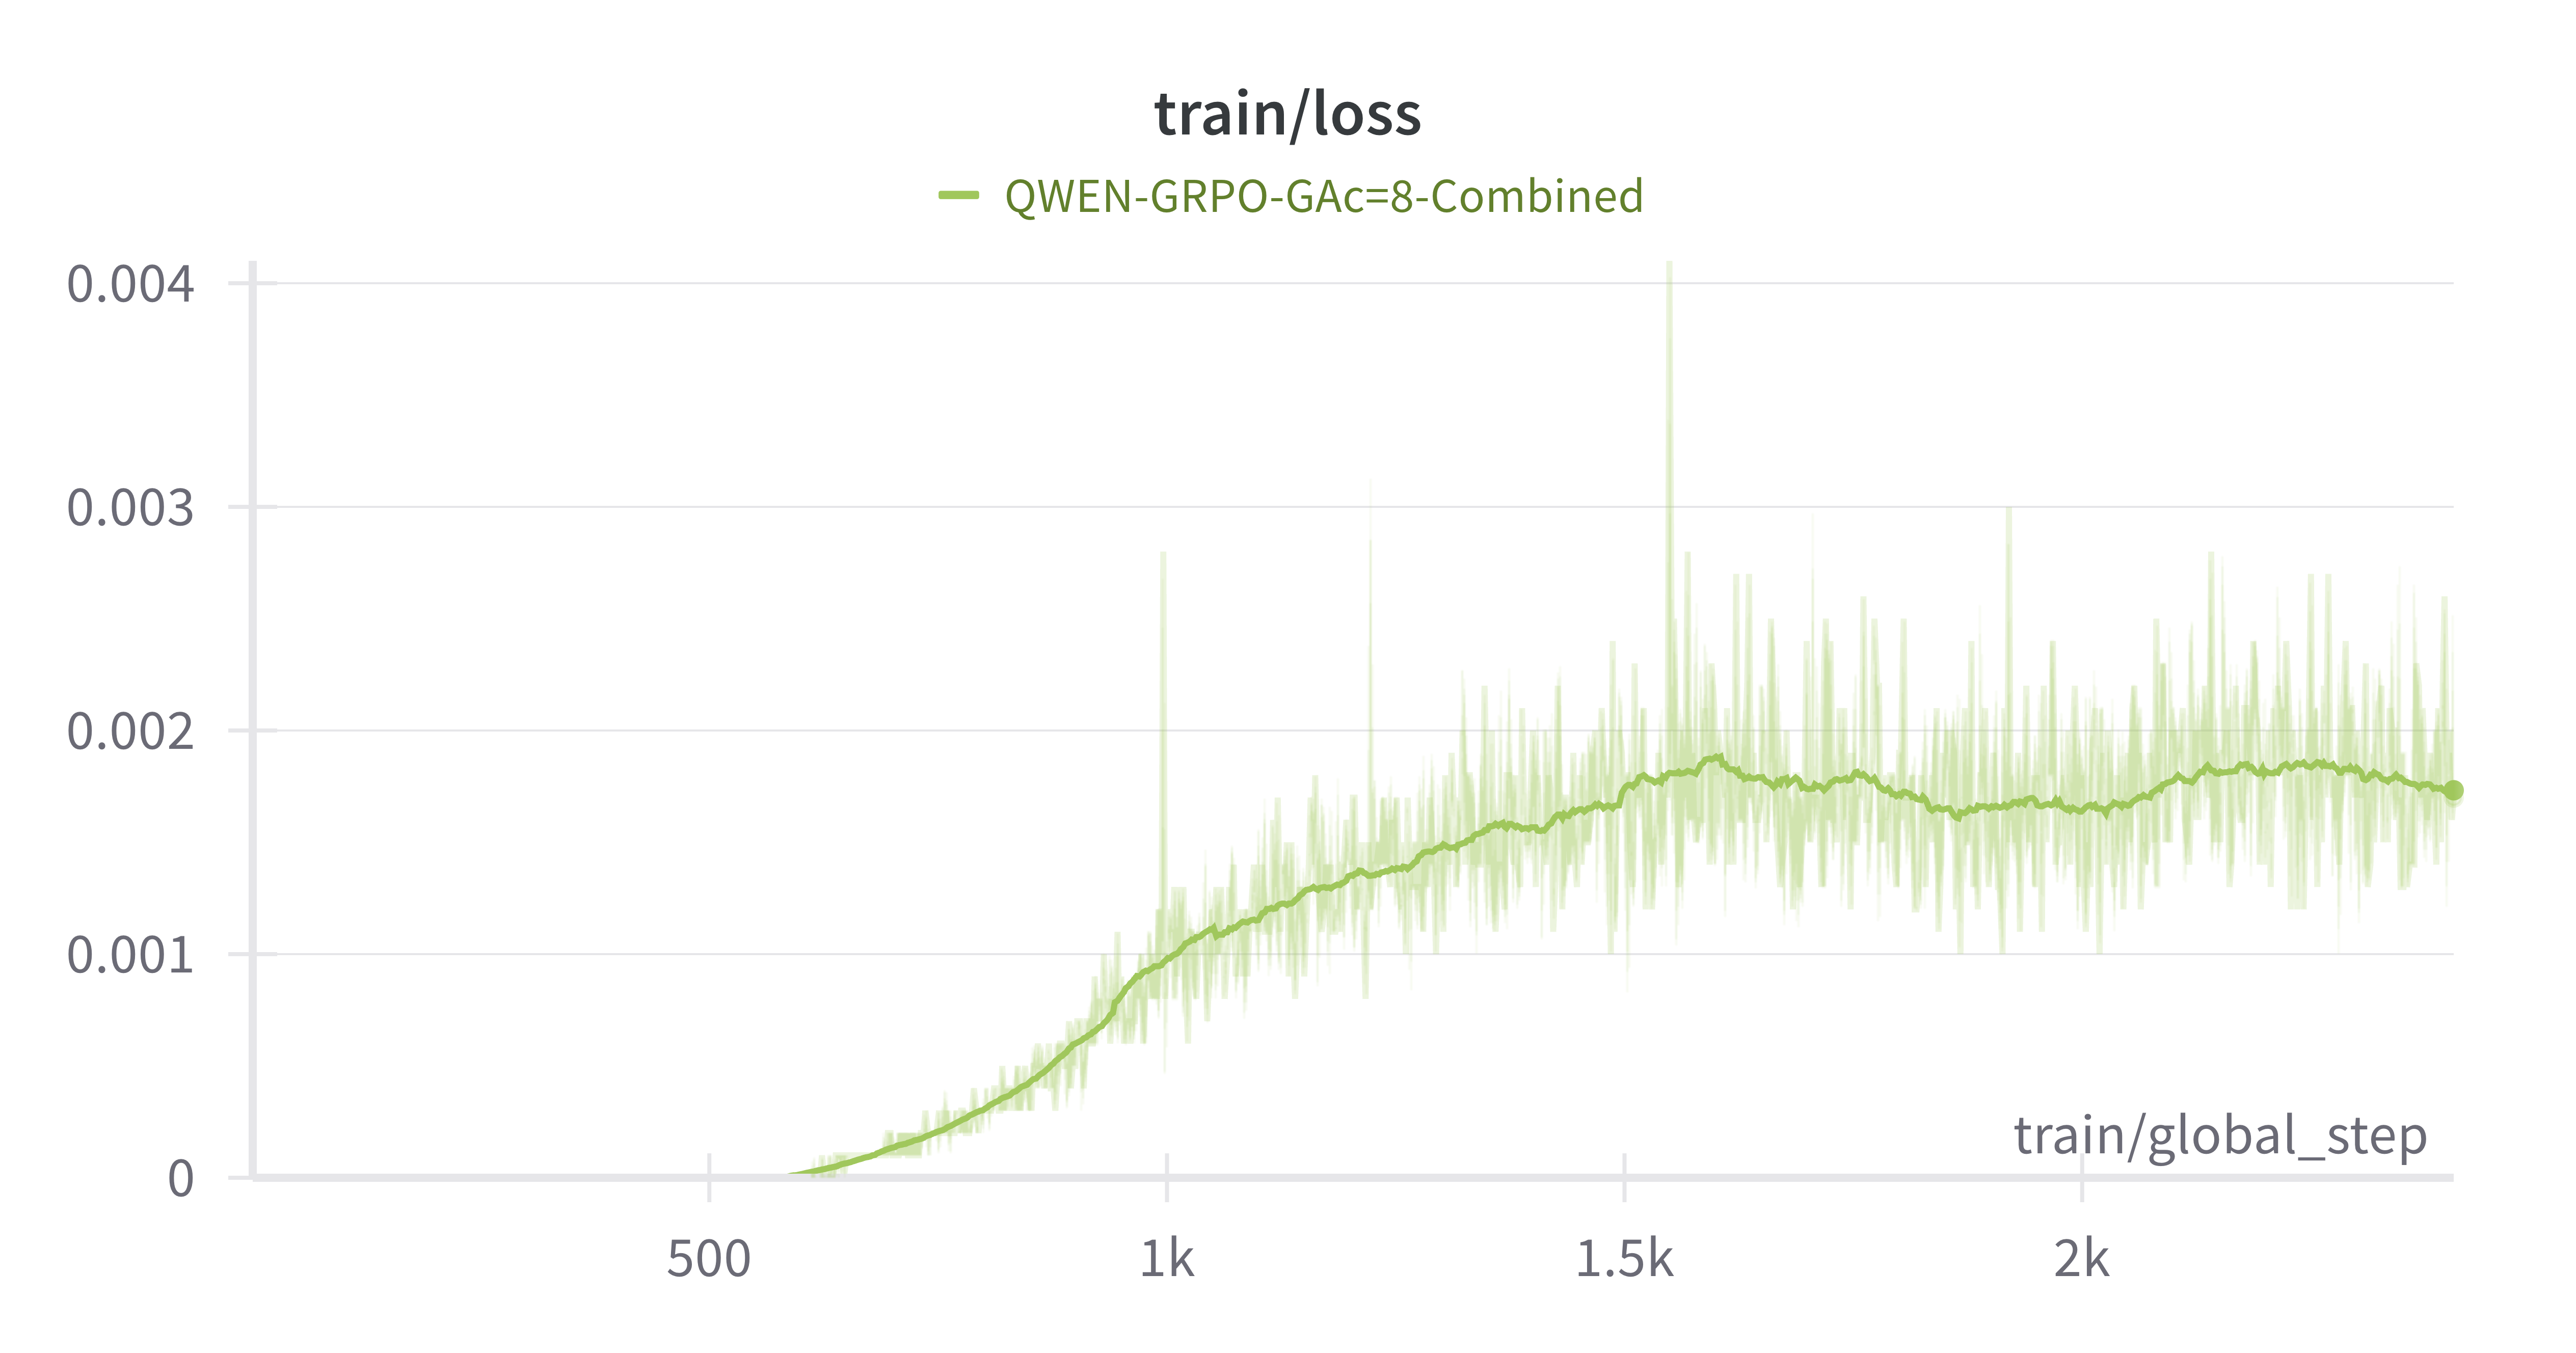
\includegraphics[width=\linewidth]{Qwen/train_loss.png} % Replace with your actual image file
        \caption*{(d) Training Loss}
        %\label{fig:qwen_loss_graph} % Optional sub-label
    \end{minipage}

    \caption{GRPO training metrics for Qwen2.5-MATH-1.5B over 6000 steps. (a) Average completion length (tokens). (b) Average correctness reward. (c) Average reasoning length (tokens, before \texttt{\textbackslash boxed\{\}}). (d) Training loss.}
    \label{fig:grpo_qwen_analysis}
\end{figure}

\begin{itemize}
    \item \textbf{Completion Length (Figure \ref{fig:grpo_qwen_analysis}a):} Analysis of the average completion length during training reveals a notable trend. In the initial stages (first ~1000 steps), the average length hovered around 320 tokens. As GRPO training progressed, guided partly by the \texttt{length\_reward\_func}, the average completion length increased substantially, eventually stabilizing near approximately 430 tokens towards the end of the training run. This increase points towards the model learning to generate more comprehensive solutions, potentially incorporating more detailed reasoning steps as intended by the reward design.

    \item \textbf{Correctness Reward (Figure \ref{fig:grpo_qwen_analysis}b):} The \texttt{correctness\_reward\_func} metric showed a dynamic pattern. While starting relatively high, it exhibited a noticeable decrease coinciding with the initial sharp increase in generation length. This suggests that as the model explored generating longer, more detailed answers, it initially struggled to maintain correctness. However, encouragingly, towards the later stages of training (after ~4000 steps), the correctness reward began a clear upward trend again. This indicates the model started to reconcile the objectives of producing detailed reasoning *and* arriving at the accurate final answer. It's possible that with further training—which was unfortunately halted after over 80 continuous hours due to exhaustion of computational lab resources—this positive trend would have continued, leading to further improvements in accuracy alongside detailed reasoning.

    \item \textbf{Reasoning Length (Figure \ref{fig:grpo_qwen_analysis}c):} Corroborating the overall completion length increase, the average reasoning length (measured as the token count *before* the final \verb|\boxed{}| answer) displayed a very similar upward trajectory. Starting around 250 tokens, it rose to stabilize near 350 tokens. This strongly indicates that the increase in overall completion length was primarily driven by more extensive step-by-step derivations, directly aligning with the goal of the \texttt{reasoning\_length\_reward\_func} to promote clearer and more detailed logical explanations preceding the final answer.

    \item \textbf{Training Loss (Figure \ref{fig:grpo_qwen_analysis}d):} The training loss presented an unusual pattern, remaining effectively zero for the initial approximately 550 steps. The exact cause for this initial zero-loss phase is unclear; it could potentially indicate an initial period where distinct preference pairs were not effectively generated or processed due to model initialization or setup characteristics, or possibly a logging artifact during the warmup phase. Subsequently, the loss rose sharply to around 0.0018 before stabilizing and remaining relatively constant for the rest of the training duration. This later behavior is more typical for policy optimization methods like GRPO, reflecting the ongoing adjustments to the policy based on the preference signals derived from the reward functions. The plateau suggests the model reached a relatively stable equilibrium point with respect to the preference data distribution generated under the configured hyperparameters and reward functions.
\end{itemize}

Overall, the GRPO training metrics for Qwen suggest that the fine-tuning process successfully encouraged the model to generate longer, more detailed reasoning steps. While this initially impacted correctness, the model showed signs of learning to balance detail with accuracy towards the end of the available training time.


\subsection{GRPO Fine-Tuning Analysis: Phi-mini-4k-instruct}

Similarly, we analyzed the training dynamics for the \texttt{unsloth/Phi-4-mini-instruct} model fine-tuned with GRPO. This analysis focuses on understanding how the model responded to the preference signals, particularly the explicit reward for adhering to the target XML output structure, alongside correctness and length objectives. Key metrics are visualized over the 14,000 training steps (Figure \ref{fig:grpo_phi_analysis}).

\begin{figure}[htbp]
    \centering
    % Define common width for 2 columns
    \newcommand{\graphwidthtwo}{0.48\textwidth}

    % First row of images
    \begin{minipage}{\graphwidthtwo}
        \centering
        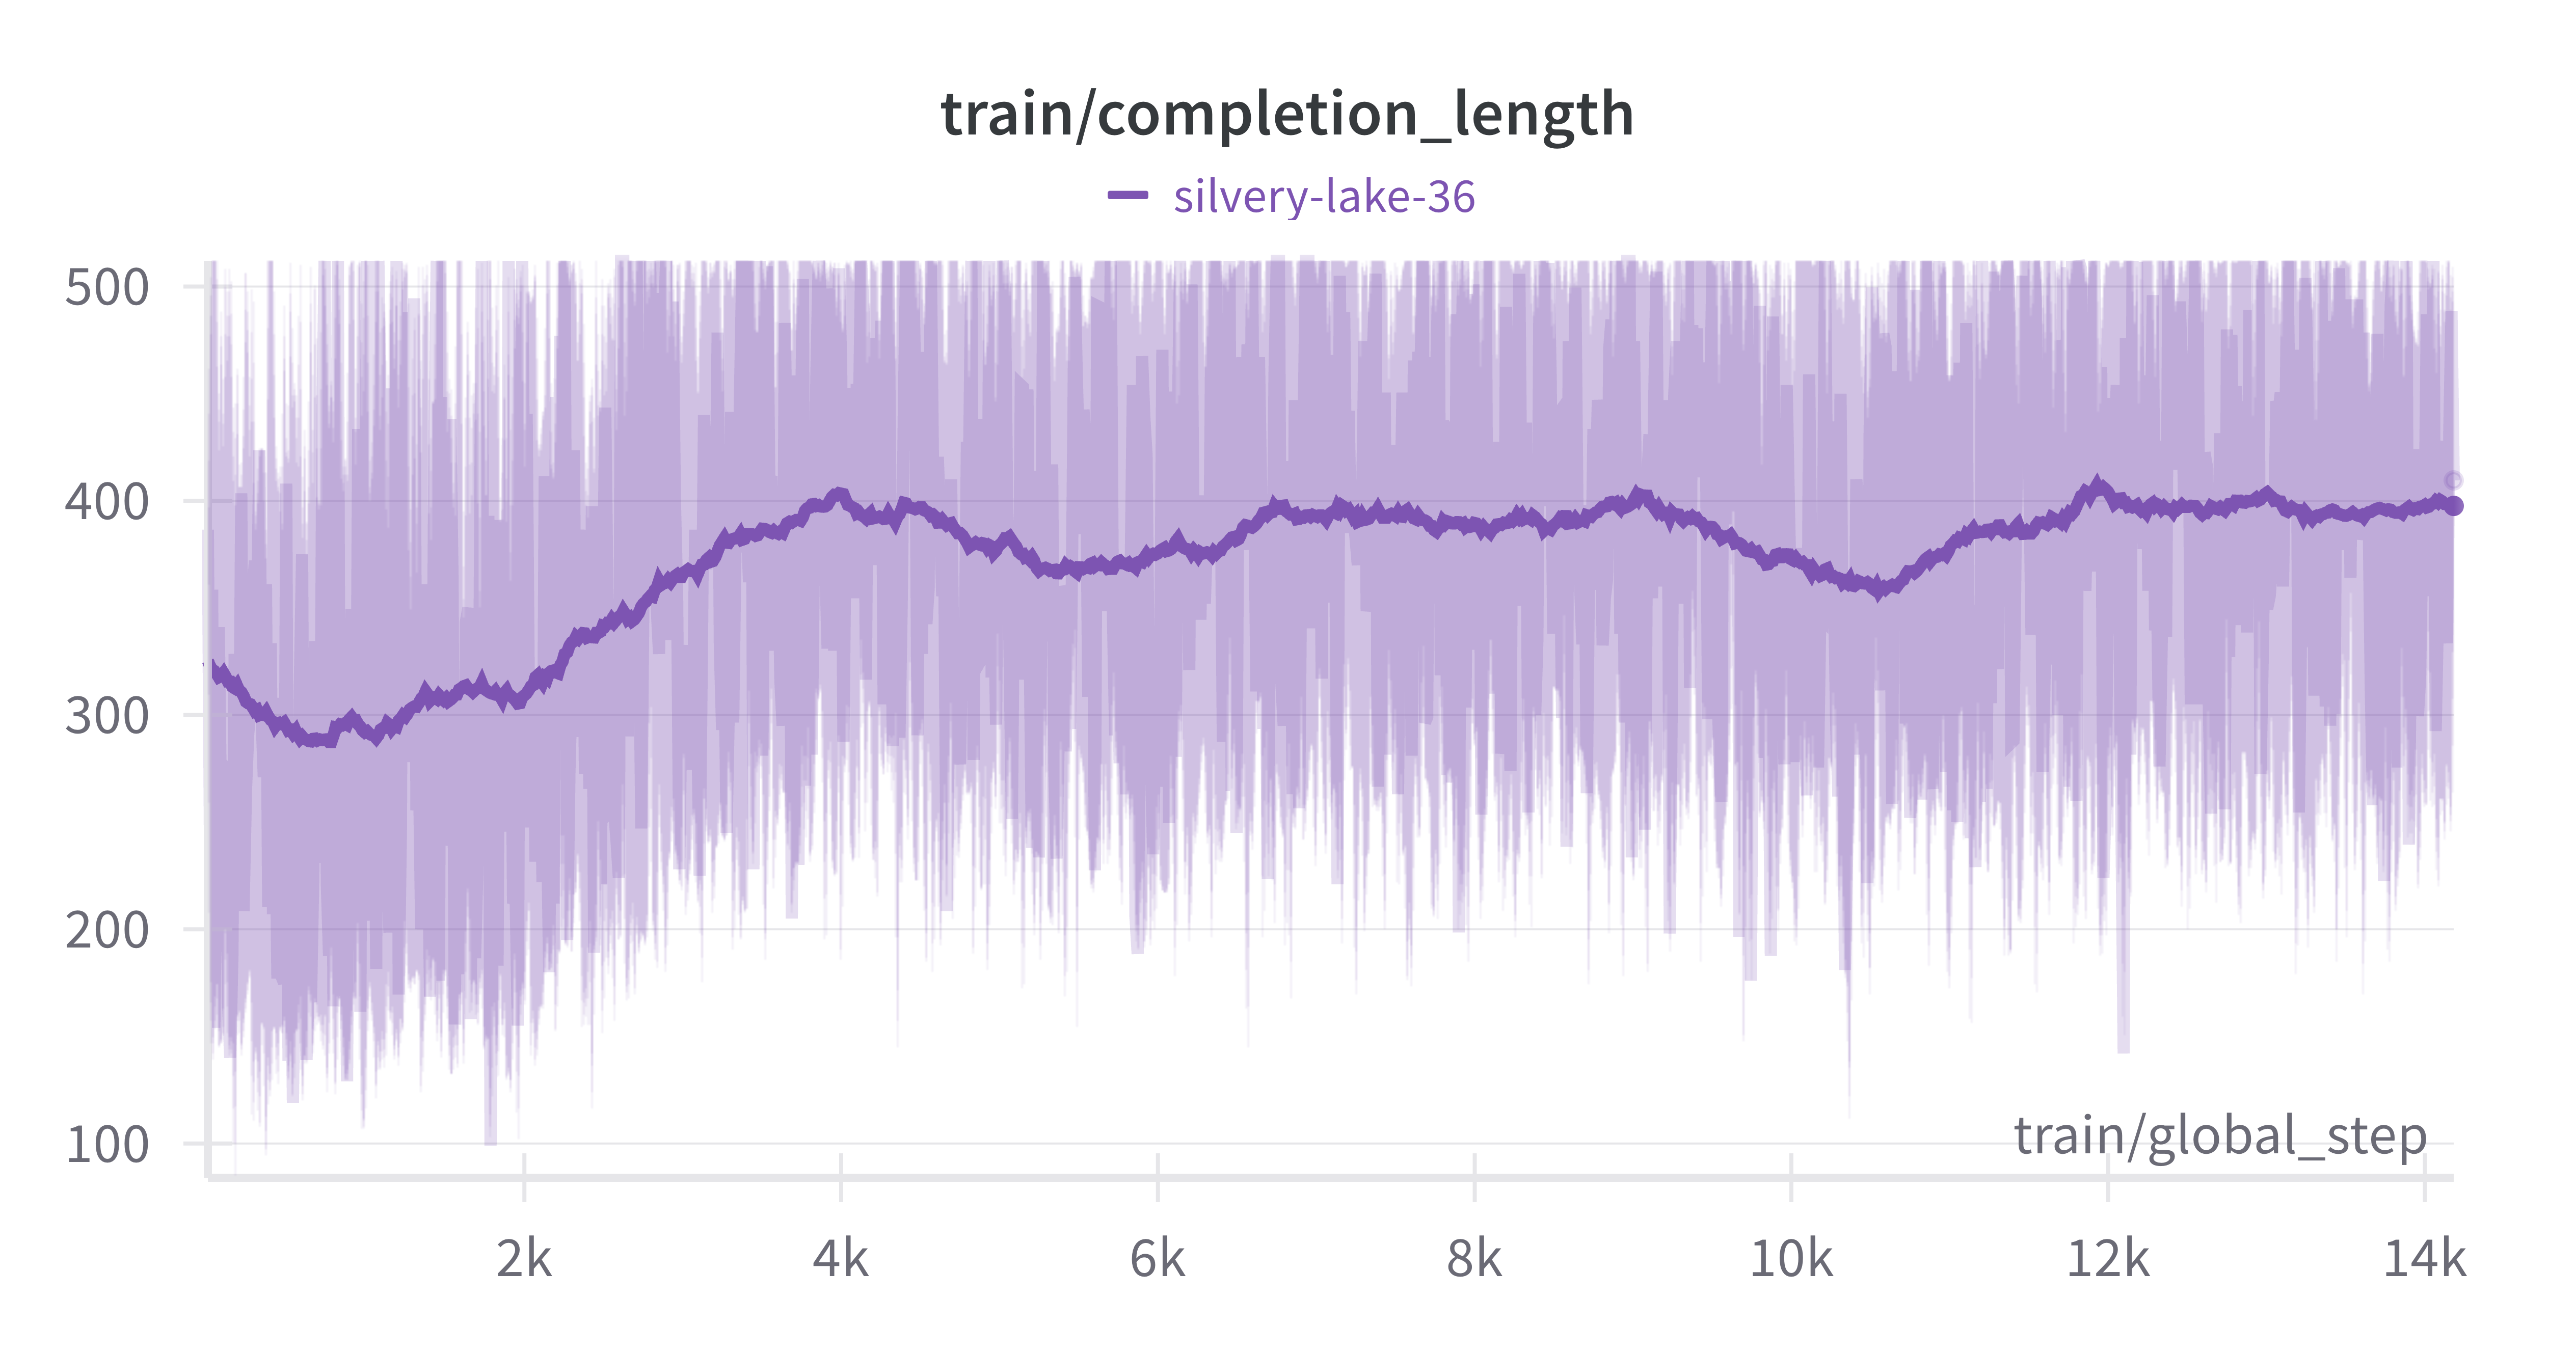
\includegraphics[width=\linewidth]{phi/completoin_length.png} % Replace with completion_length.png
        \caption*{(a) Completion Length}
    \end{minipage}\hfill
    \begin{minipage}{\graphwidthtwo}
        \centering
        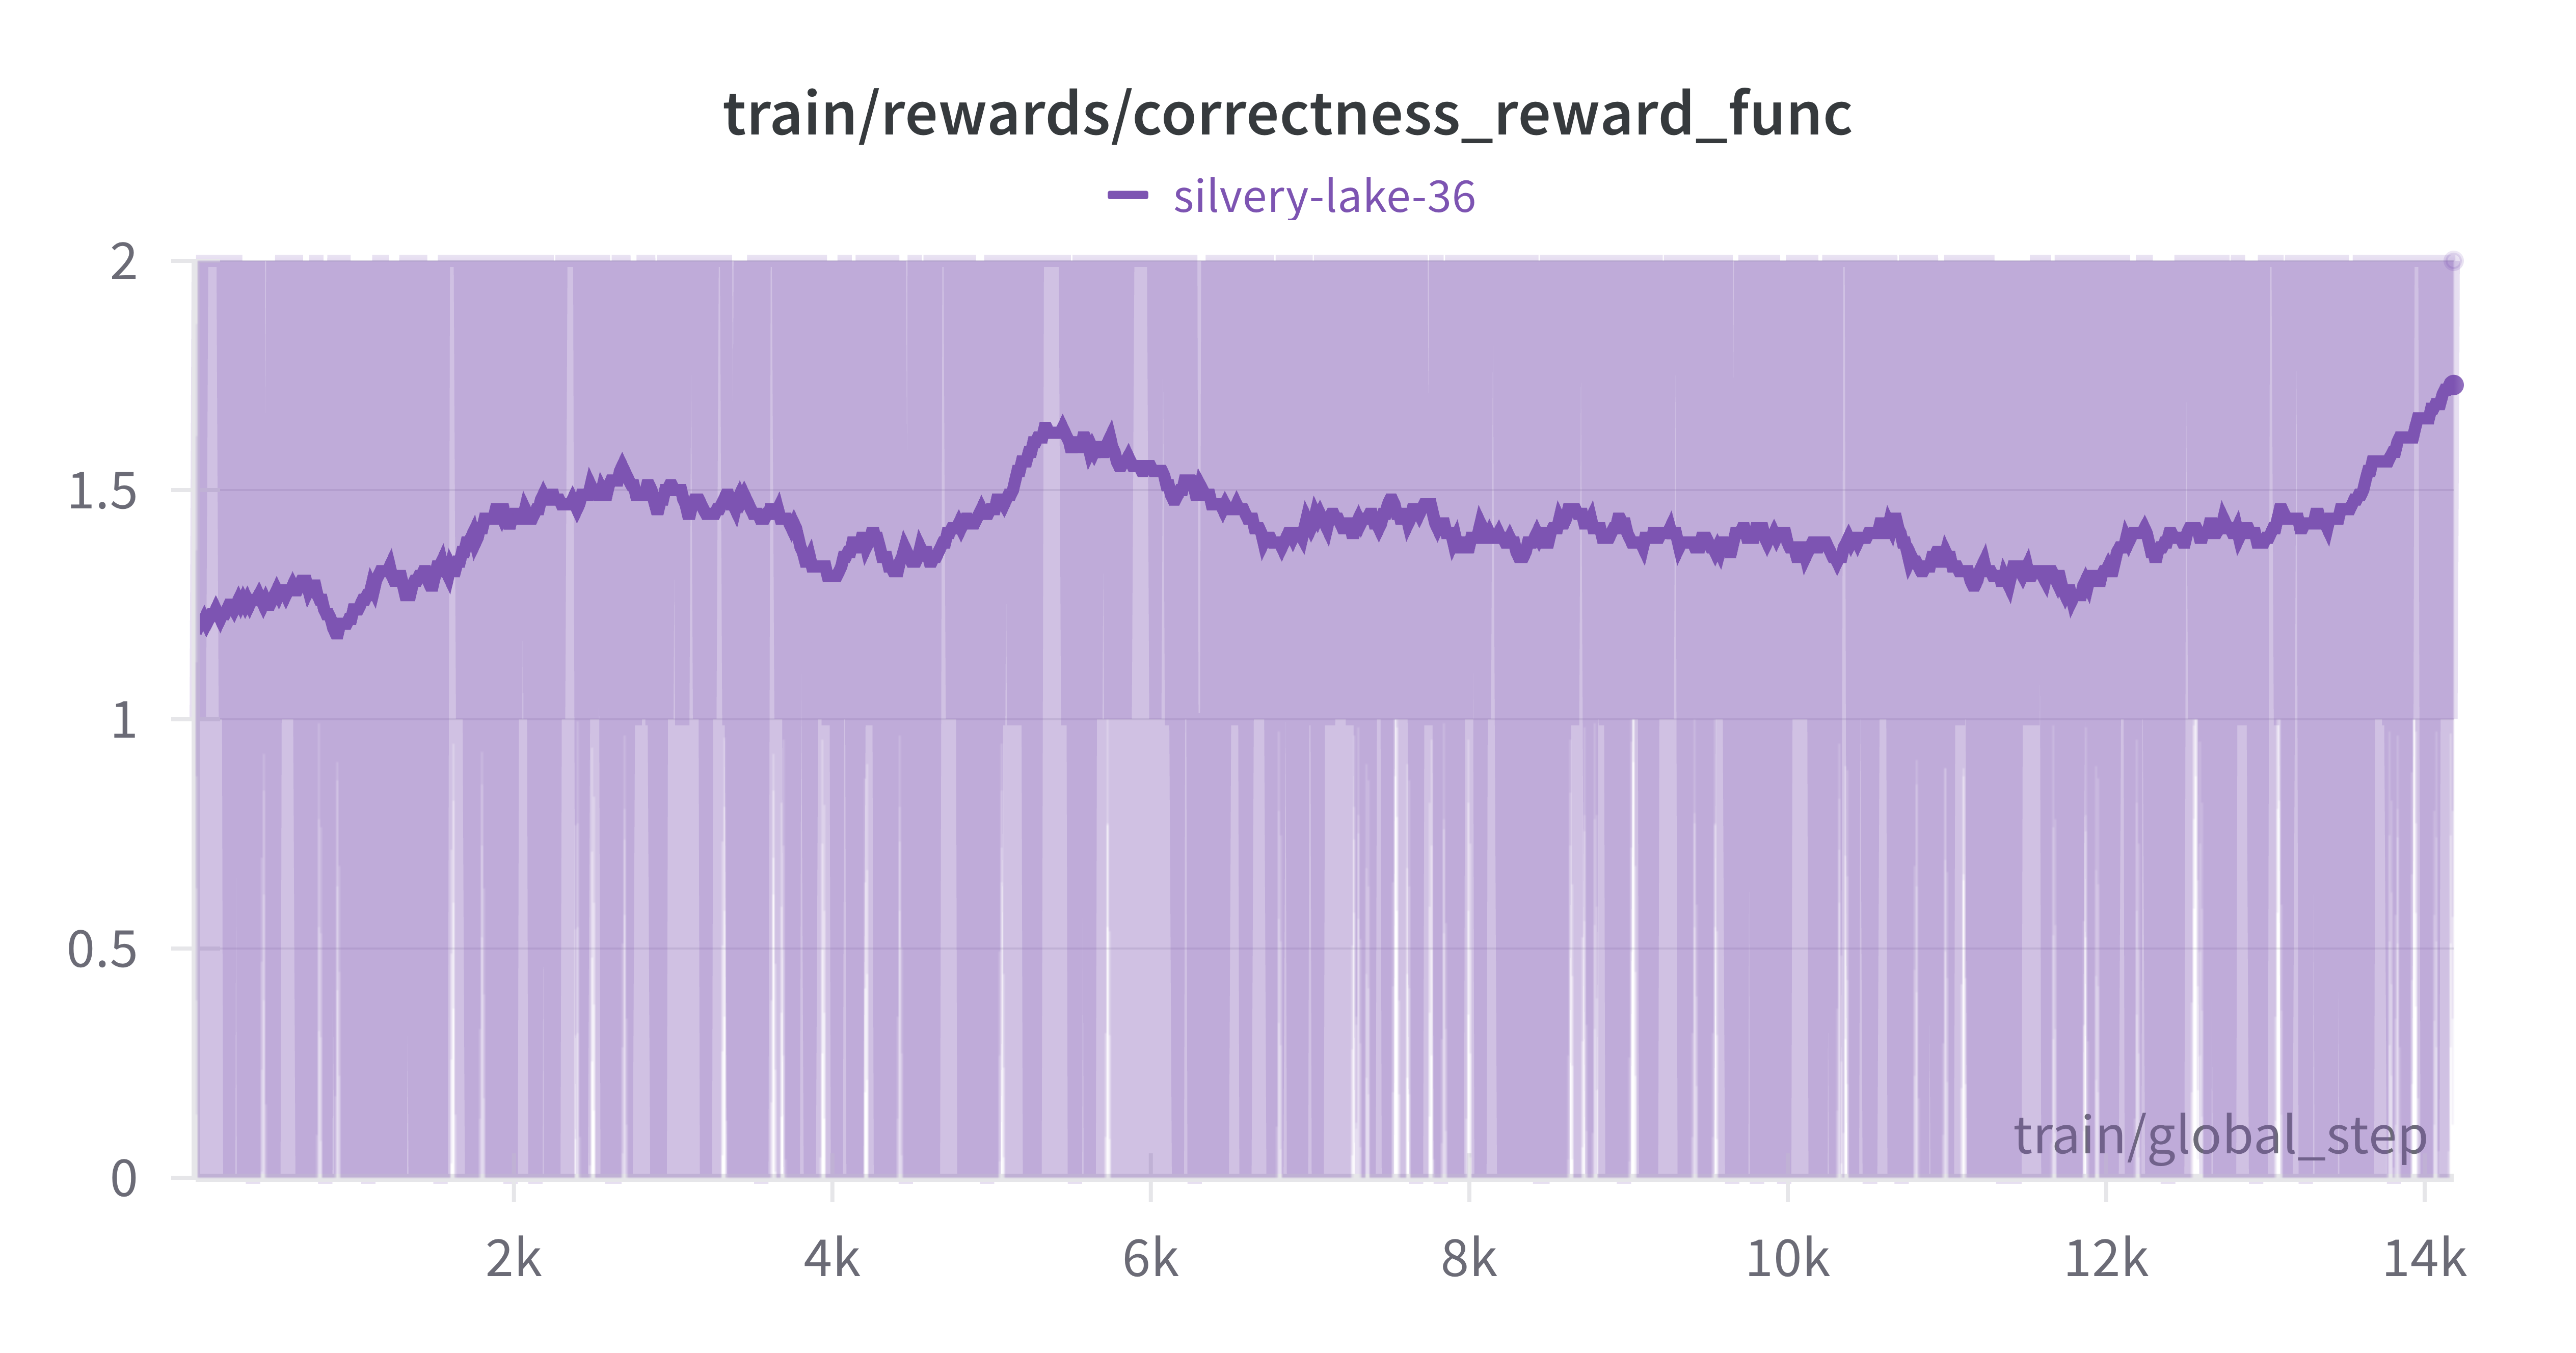
\includegraphics[width=\linewidth]{phi/correctness_reward.png} % Replace with correctness_reward_func.png
        \caption*{(b) Correctness Reward}
    \end{minipage}

    \vspace{1em} % Add vertical space between rows

    % Second row of images
    \begin{minipage}{\graphwidthtwo}
        \centering
        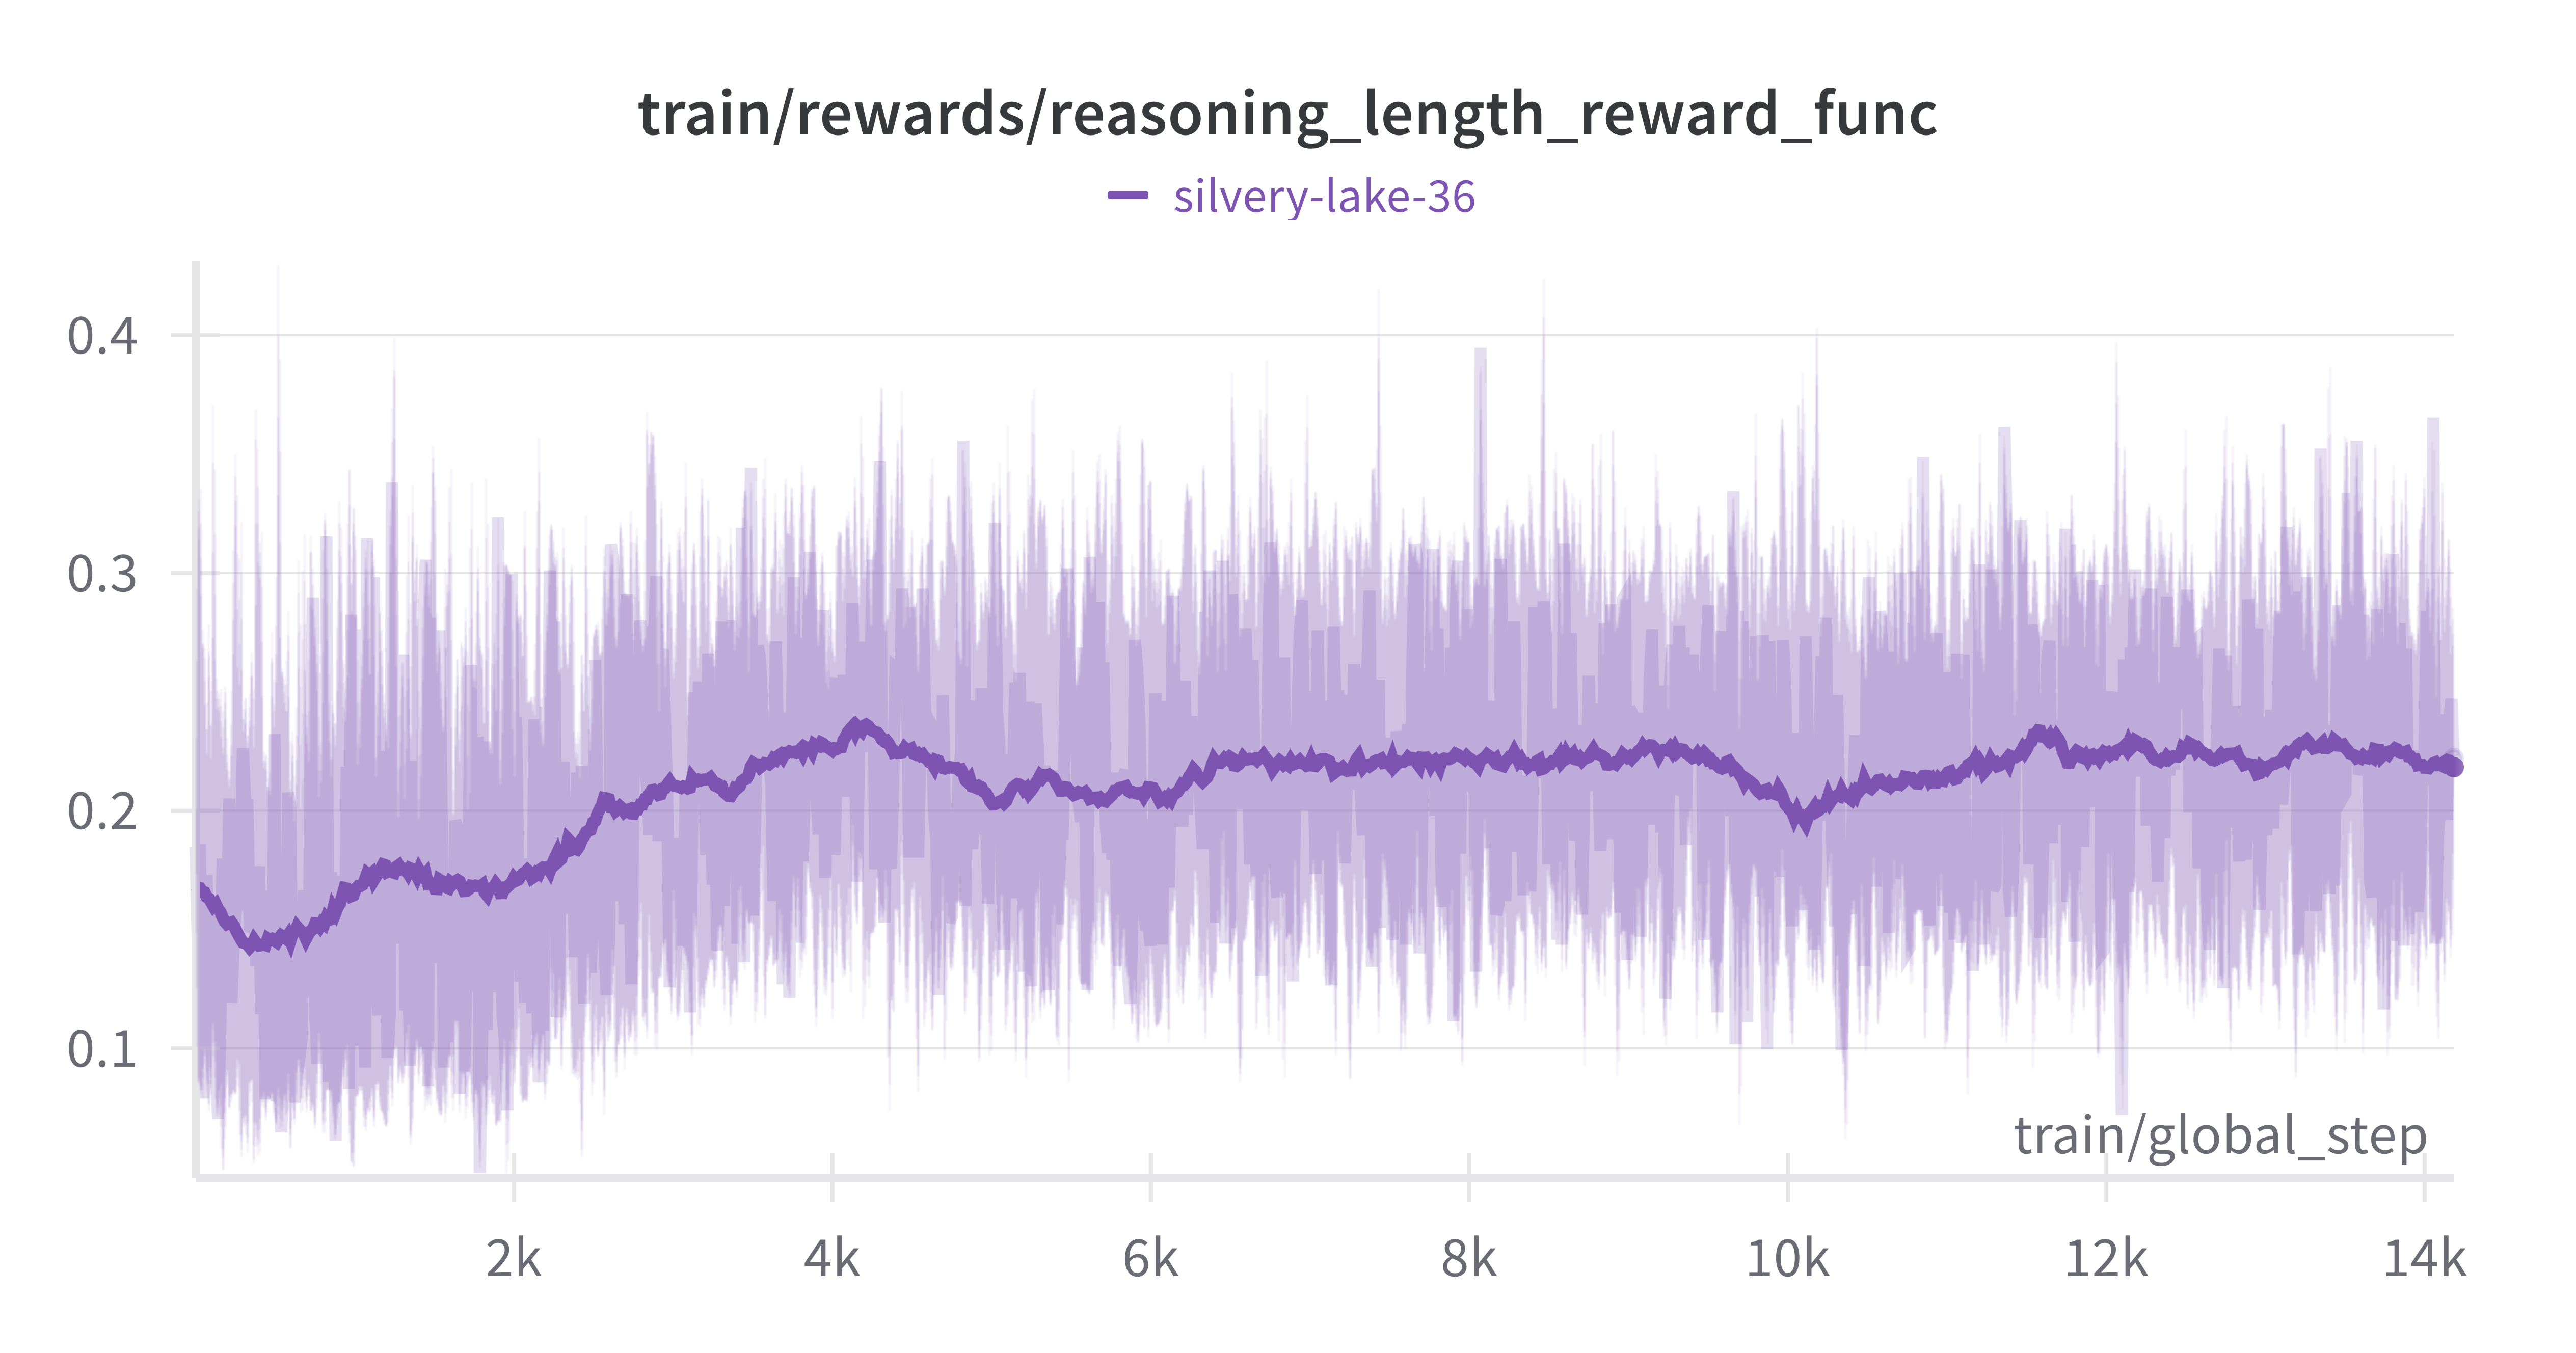
\includegraphics[width=\linewidth]{phi/reasoning_length_reward.png} % Replace with reasoning_length_reward_func.png
        \caption*{(c) Reasoning Length Reward}
    \end{minipage}\hfill
    \begin{minipage}{\graphwidthtwo}
        \centering
        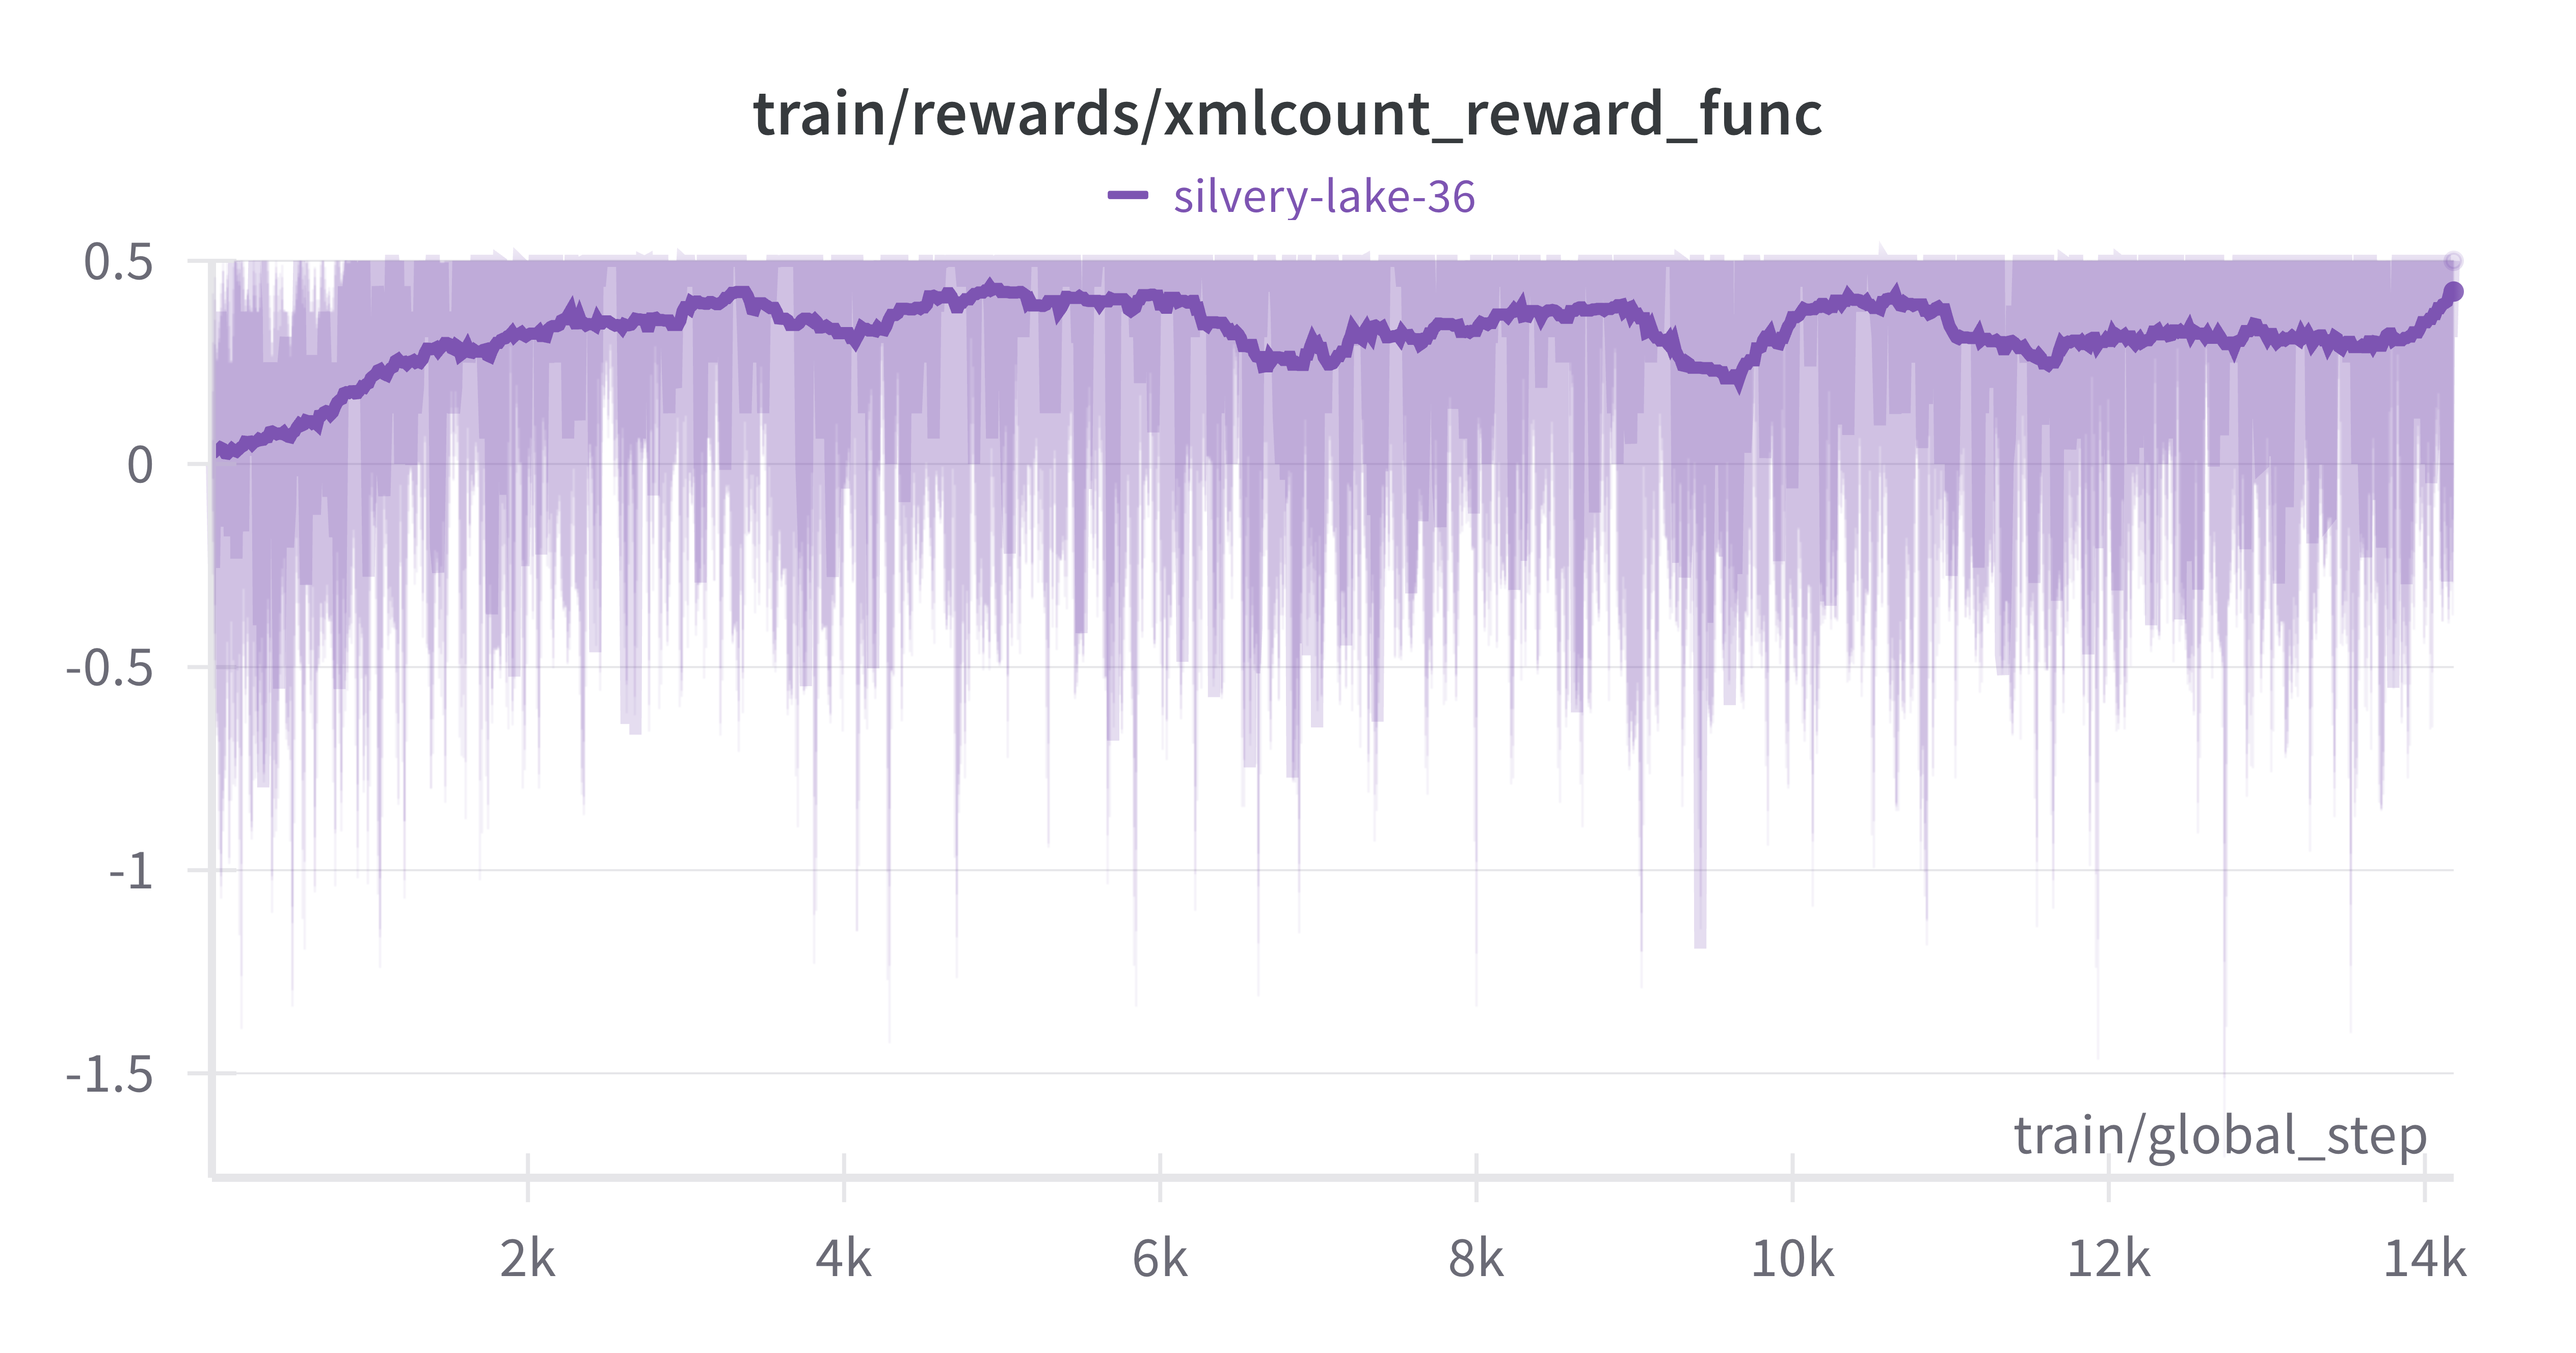
\includegraphics[width=\linewidth]{phi/XML_Count_reward.png} % Replace with xmlcount_reward_func.png
        \caption*{(d) XML Count Reward}
    \end{minipage}

    \vspace{1em} % Add vertical space between rows

    % Third row of images
    \begin{minipage}{\graphwidthtwo}
        \centering
        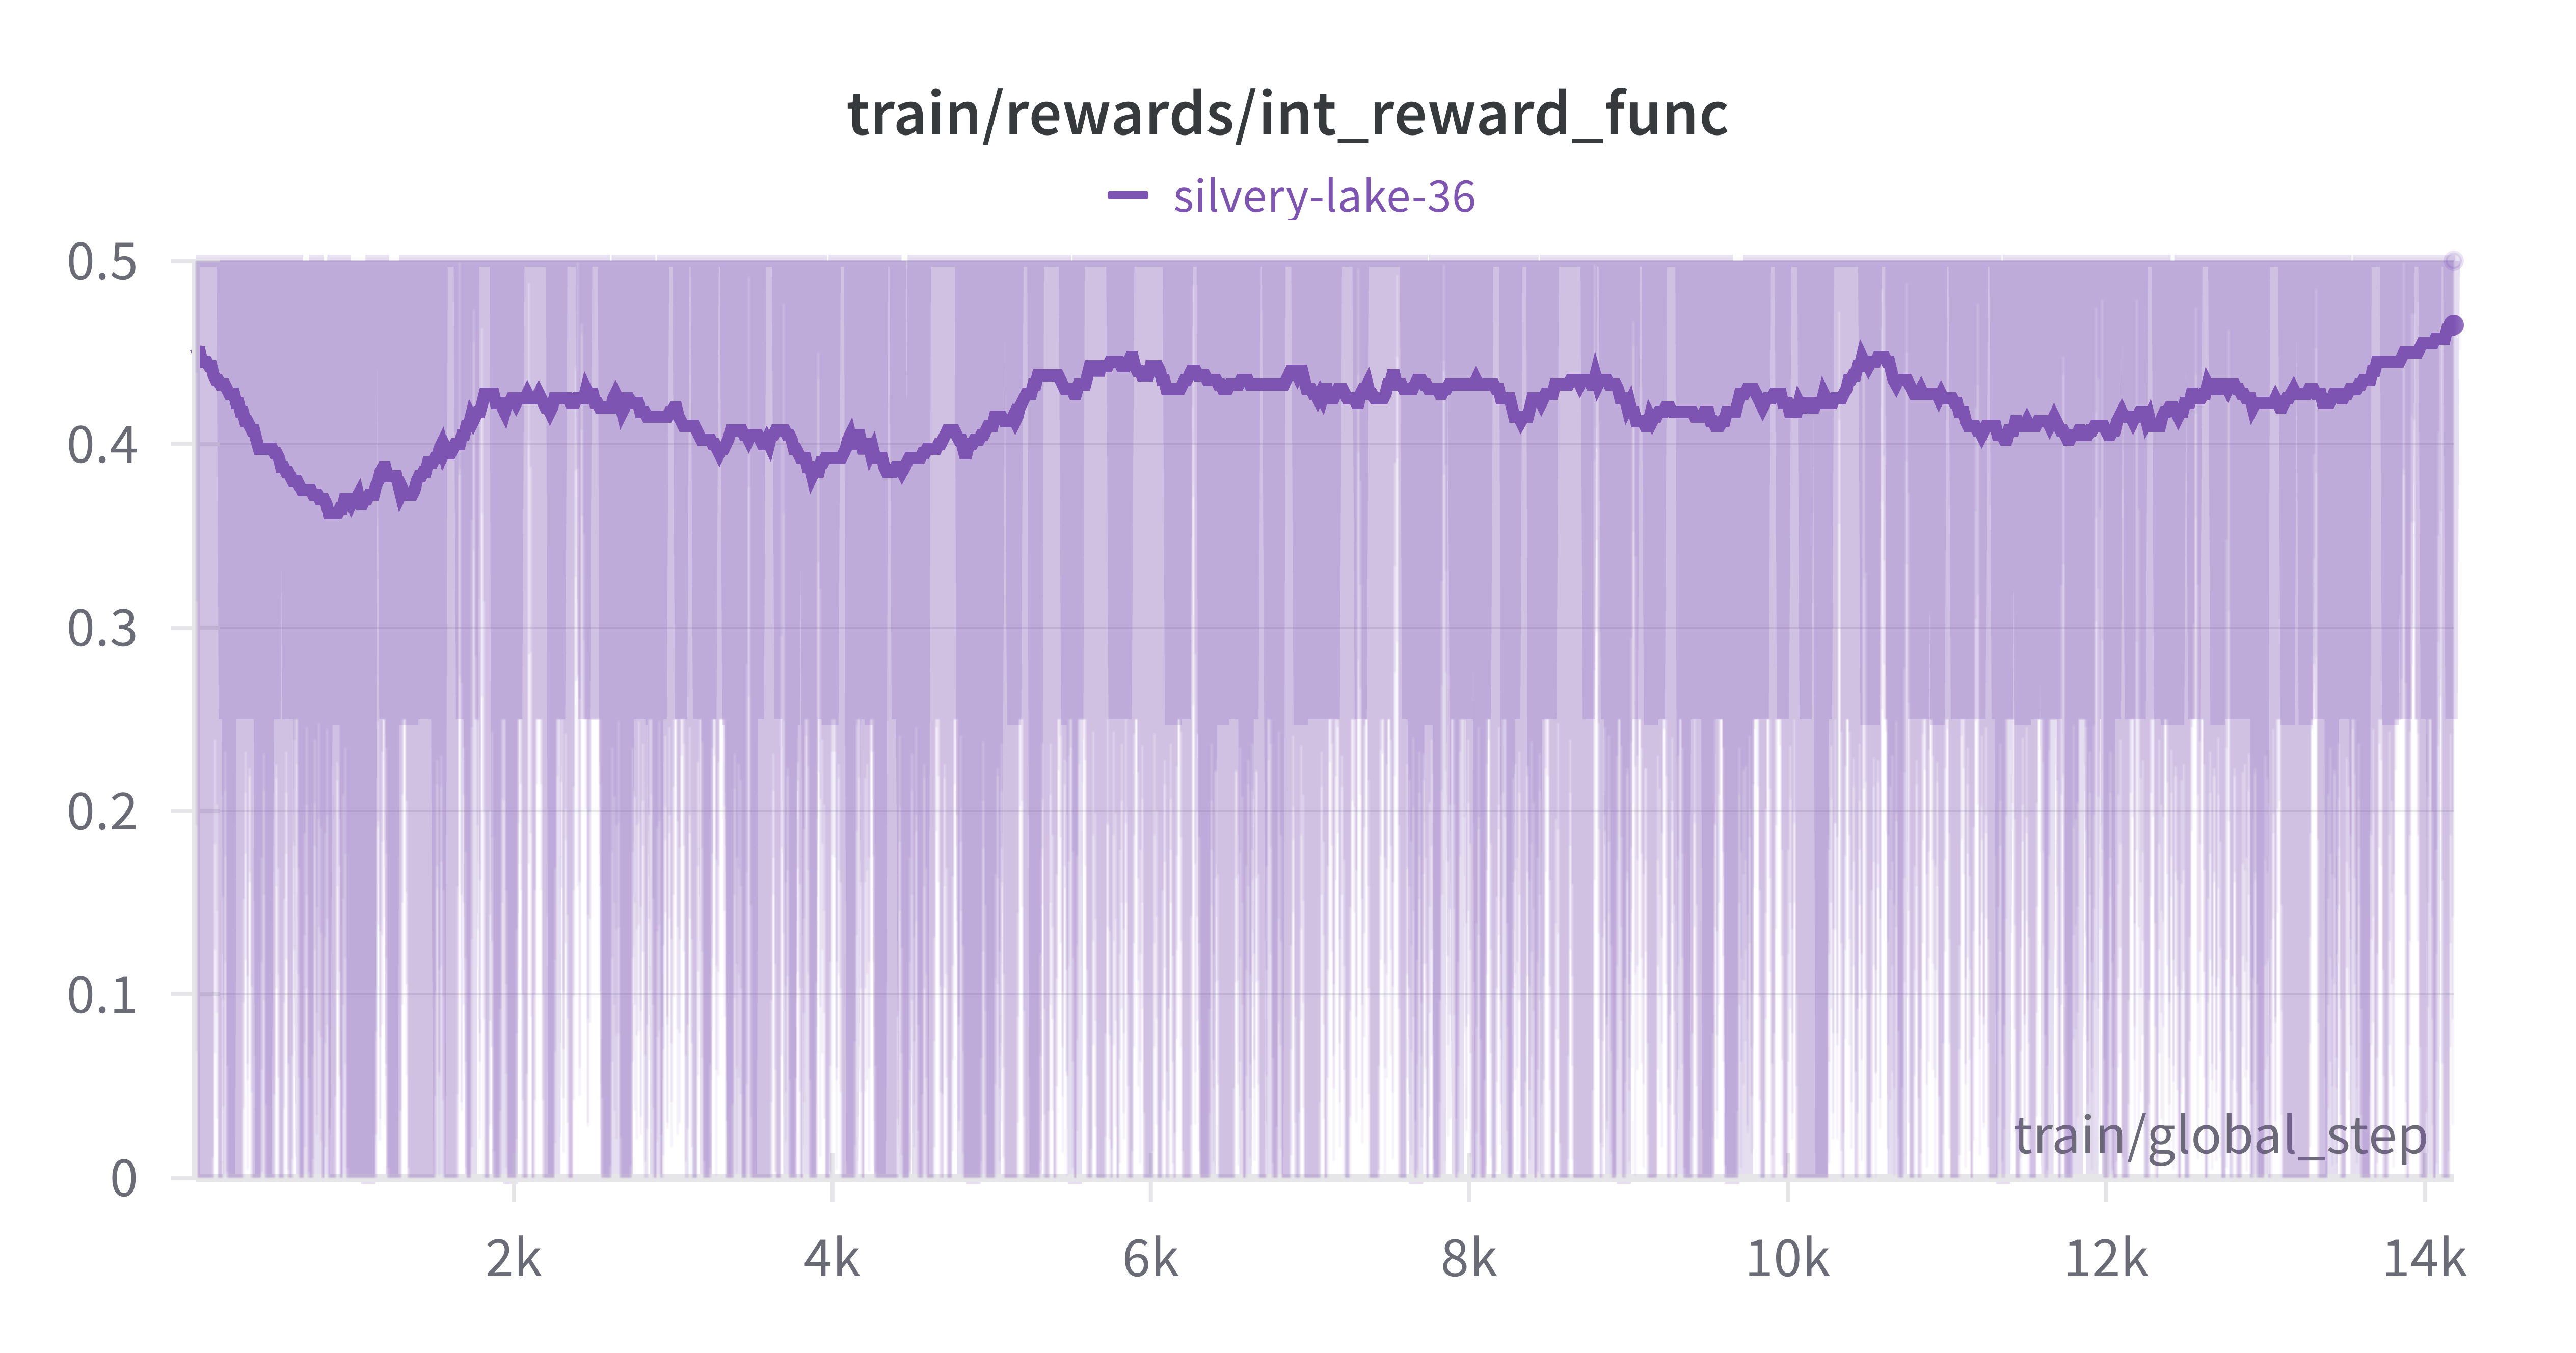
\includegraphics[width=\linewidth]{phi/int_reward.png} % Replace with int_reward_func.png
        \caption*{(e) Integer Format Reward}
    \end{minipage}\hfill
    \begin{minipage}{\graphwidthtwo}
        \centering
        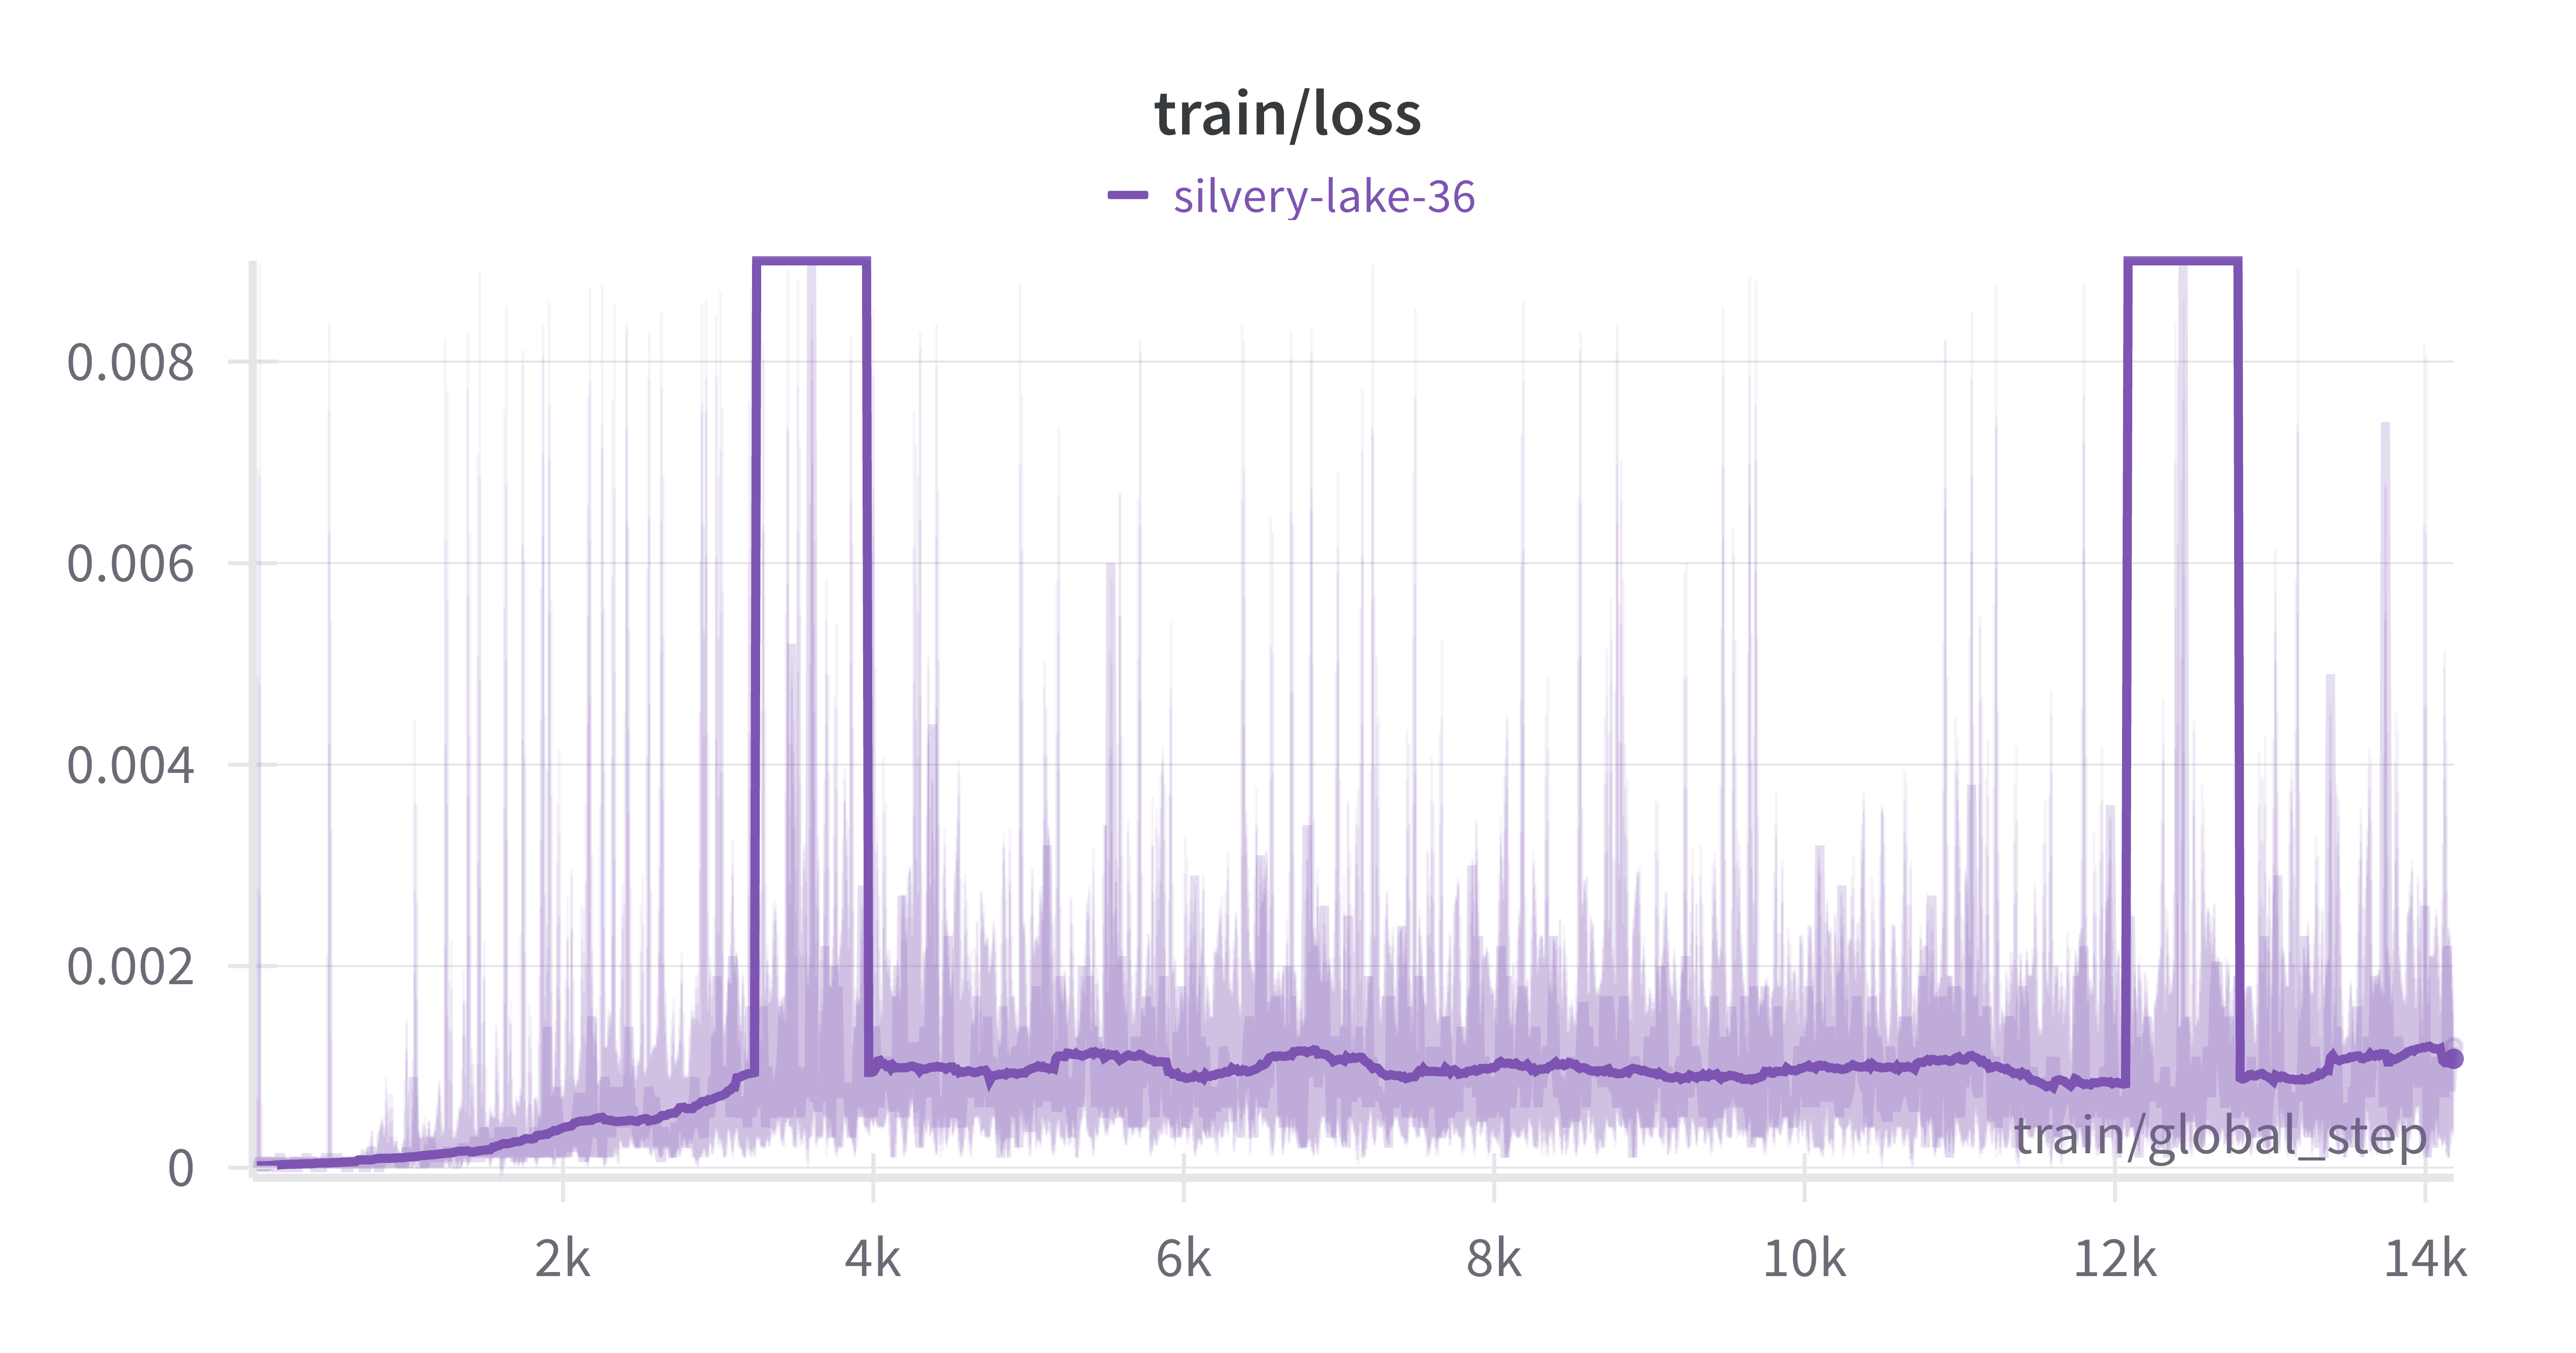
\includegraphics[width=\linewidth]{phi/train_loss.png} % Replace with train_loss.png
        \caption*{(f) Training Loss}
    \end{minipage}


    \caption{GRPO training metrics for Phi-mini-4k-instruct over 14,000 steps. (a) Average completion length. (b) Average correctness reward. (c) Average reasoning length reward. (d) Average XML structure adherence reward. (e) Average integer format reward. (f) Training loss.}
    \label{fig:grpo_phi_analysis}
\end{figure}

\begin{itemize}
    \item \textbf{Completion Length (Figure \ref{fig:grpo_phi_analysis}a):} The average completion length for Phi-mini shows an initial increase, rising from roughly 300 tokens to a peak near 400 tokens around the 4000-step mark. Subsequently, it exhibits more fluctuation and a slight downward trend, stabilizing closer to 380-390 tokens towards the end. Unlike the steady increase seen with Qwen, this suggests a more complex interplay between generating detailed reasoning (encouraged by length rewards) and adhering to the specific XML structure and correctness constraints. The model might be learning to be more concise once the structural and correctness requirements are better met.

    \item \textbf{Correctness Reward (Figure \ref{fig:grpo_phi_analysis}b):} The correctness reward demonstrates a strong and fairly consistent upward trend throughout the training. Starting around 1.2, it climbs steadily, surpassing 1.6 and showing continued improvement towards the end, approaching 1.8. This is a very positive signal, indicating that the fine-tuning process was effective in significantly enhancing the model's ability to arrive at the correct final answer. The robust answer extraction logic (\texttt{extract\_xml\_answer}) likely contributed to accurately rewarding correct answers regardless of minor formatting variations.

    \item \textbf{Reasoning Length Reward (Figure \ref{fig:grpo_phi_analysis}c):} The reward associated with the length of the reasoning part (before the answer tag) shows a clear learning curve. It increases from about 0.15 to approximately 0.22 by the 4000-step mark and then largely stabilizes, with minor fluctuations. This indicates the model successfully learned to produce more elaborate reasoning steps, fulfilling the objective of this reward component, and found a consistent level of detail suitable within the overall generation process.

    \item \textbf{XML Count Reward (Figure \ref{fig:grpo_phi_analysis}d):} This metric, specific to the Phi-mini fine-tuning, tracks adherence to the desired XML structure. Starting near zero, it shows a significant and steady increase, plateauing around 0.4-0.45 for the latter half of training. This strongly suggests that the \texttt{xmlcount\_reward\_func} was highly effective in guiding the model to generate responses conforming to the target format (e.g., using `<reasoning>`, `<answer>` tags correctly). The plateau indicates the model consistently incorporated most of the required structural elements.

    \item \textbf{Integer Format Reward (Figure \ref{fig:grpo_phi_analysis}e):} The reward for producing clean integer answers remained relatively high and stable throughout training. After a small initial dip, it hovered consistently around 0.45. This suggests the model maintained its ability to output integers correctly when needed, potentially aided by the clear structure provided by the XML tags for isolating the final answer.

    \item \textbf{Training Loss (Figure \ref{fig:grpo_phi_analysis}f):} The training loss for Phi-mini starts near zero, increases rapidly in the first few hundred steps, and then settles into a relatively low average value (around 0.001). Unlike the initial zero-loss phase observed in the Qwen run, Phi's loss becomes positive almost immediately. However, the loss graph exhibits significant volatility with large, sharp spikes occurring periodically (e.g., around 3.5k and 12k steps), even though the smoothed average remains low and stable. These spikes might represent moments where the model encountered particularly challenging preference distinctions or made significant policy adjustments. Overall, the low average loss indicates effective convergence of the GRPO algorithm.
\end{itemize}

In summary, the GRPO fine-tuning for Phi-mini appears successful in simultaneously improving correctness, encouraging detailed reasoning, and notably, enforcing adherence to a specific structured XML output format. The model learned to balance these objectives, demonstrating the flexibility of GRPO in optimizing for multiple, potentially conflicting, criteria.

\subsection{Results and Analyses: Post-GRPO Performance}

Following the GRPO fine-tuning process detailed in the previous sections, we evaluated the final performance of the optimized Qwen2.5-MATH-1.5B and Phi-mini-4k-instruct models on the GSM8K and MATH 500 datasets. The goal was to quantify the improvements achieved through preference optimization and compare the capabilities of these fine-tuned SLMs against each other, their respective baselines, and the high-performance Gemini-2.0-Flash benchmark.

Table \ref{tab:grpo_performance} presents the accuracy scores achieved by the models after GRPO fine-tuning.

\begin{table}[htbp]
\centering
\caption{Performance of SLMs after GRPO Fine-Tuning.}
\label{tab:grpo_performance}
\begin{tabular}{@{}l c c@{}}
\toprule
\textbf{Model (GRPO Fine-Tuned)} & \textbf{GSM8K Acc.} & \textbf{MATH 500 Acc.} \\
\midrule
Qwen2.5-MATH-1.5B (4-bit) & 78.6\% & 29.0\% \\
Phi-mini-4k-instruct (4-bit) & 83.33\% & 33.5\% \\
\bottomrule
\end{tabular}
\end{table}

\subsection{Analysis of Fine-Tuning Impact}

A comparative analysis of these results reveals several key insights:

\begin{itemize}
    \item \textbf{Improvement over Baselines:} Both models showed clear gains from GRPO fine-tuning.
        \begin{itemize}
            \item \textbf{Qwen2.5-MATH:} The GRPO fine-tuned Qwen model improved its GSM8K accuracy from 76.80\% to 78.6\% (+1.8 percentage points) and its MATH 500 accuracy from 24.43\% to 29.0\% (+4.57 percentage points). The larger gain on the more complex MATH dataset suggests the fine-tuning was particularly beneficial for challenging reasoning tasks, aligning with the training analysis that showed improving correctness alongside detailed reasoning.
            \item \textbf{Phi-mini-4k-instruct:} Phi-mini demonstrated substantial improvement. Its GSM8K accuracy rose from 78.04\% to 83.33\% (+5.29 percentage points), and its MATH 500 accuracy saw a very significant jump from 18.85\% to 33.5\% (+14.65 percentage points). This dramatic improvement on MATH 500 highlights the effectiveness of the GRPO strategy combined with tailored reward functions (including XML formatting guidance) in unlocking the reasoning potential of this model.
        \end{itemize}

    \item \textbf{Comparison between Fine-Tuned SLMs:}
        \begin{itemize}
            \item After GRPO fine-tuning, Phi-mini-4k-instruct clearly outperformed Qwen2.5-MATH-1.5B on both benchmarks.
            \item On GSM8K, Phi-mini (83.33\%) scored 4.73 percentage points higher than Qwen (78.6\%).
            \item On MATH 500, Phi-mini (33.5\%) scored 4.5 percentage points higher than Qwen (29.0\%).
            \item This suggests that either Phi-mini possesses inherently stronger reasoning capabilities that were better surfaced by GRPO, or that the combination of GRPO with the specific XML-focused reward strategy used for Phi was more effective than the strategy applied to Qwen. The strong correctness trend seen during Phi's training supports this.
        \end{itemize}

    \item \textbf{Comparison against High-Performance Baseline (Gemini-2.0-Flash):}
        \begin{itemize}
            \item \textbf{GSM8K:} Both fine-tuned SLMs surpassed the baseline performance of Gemini-2.0-Flash (72.78\%). Qwen-GRPO (78.6\%) exceeded it by 5.82 points, and Phi-GRPO (83.33\%) surpassed it by a significant 10.55 points. This shows that GRPO-tuned SLMs can be highly competitive or even superior on foundational multi-step arithmetic reasoning compared to a strong generalist model.
            \item \textbf{MATH 500:} On the more demanding MATH 500 dataset, the results are more nuanced. Qwen-GRPO (29.0\%) still lagged behind Gemini (33.69%). However, the fine-tuned Phi-mini-GRPO (33.5\%) achieved performance almost identical to Gemini-2.0-Flash (only 0.19 percentage points lower). This is a remarkable result, demonstrating that a 4B parameter SLM, when appropriately fine-tuned with preference optimization, can reach parity with a much larger, state-of-the-art model on a complex mathematical reasoning benchmark.
        \end{itemize}
\end{itemize}

In summary, the GRPO fine-tuning proved effective in enhancing the mathematical reasoning capabilities of both SLMs. Phi-mini emerged as the stronger performer post-tuning, achieving parity with Gemini-2.0-Flash on the challenging MATH 500 dataset and surpassing it on GSM8K. Qwen-MATH also showed clear improvements, particularly on MATH 500, and surpassed Gemini on GSM8K. These results underscore the potential of efficient preference optimization techniques like GRPO to unlock strong reasoning performance in resource-constrained SLMs, making them viable alternatives to larger models for specific domains.



\begin{table}[htbp]
    \centering
    \caption{Summary of Performance Improvement after GRPO Fine-Tuning}
    \label{tab:summary_comparison}
    \sisetup{round-mode=places, round-precision=2, table-format=2.2}
    
    % GSM8K Accuracy Table
    \begin{subtable}{\linewidth}
    \centering
    \caption{GSM8K Accuracy (\%)}
    \begin{tabular}{@{}l
                    S[table-format=2.2]
                    S[table-format=2.2]
                    S[table-format=2.2, color=improvementgreen, detect-weight]
                    @{}}
    \toprule
    \textbf{Model} & {Baseline} & {GRPO Tuned} & {Improvement (pp)} \\
    \midrule
    Qwen2.5-MATH-1.5B (4-bit)     & 76.80 & 78.60 & \bfseries +1.80 \\
    Phi-mini-4k-instruct (4-bit)  & 78.04 & 83.33 & \bfseries +5.29 \\
    \bottomrule
    \end{tabular}
    \end{subtable}
    
    \vspace{1em} % Add vertical spacing
    
    % MATH 500 Accuracy Table
    \begin{subtable}{\linewidth}
    \centering
    \caption{MATH 500 Accuracy (\%)}
    \begin{tabular}{@{}l
                    S[table-format=2.2]
                    S[table-format=2.2]
                    S[table-format=2.2, color=improvementgreen, detect-weight]
                    @{}}
    \toprule
    \textbf{Model} & {Baseline} & {GRPO Tuned} & {Improvement (pp)} \\
    \midrule
    Qwen2.5-MATH-1.5B (4-bit)     & 24.43 & 29.00 & \bfseries +4.57 \\
    Phi-mini-4k-instruct (4-bit)  & 18.85 & 33.50 & \bfseries +14.65 \\
    \bottomrule
    \end{tabular}
    \end{subtable}
    
    \vspace{0.5em}
    \footnotesize\raggedright
    pp: percentage points. Improvements are highlighted in \textcolor{improvementgreen}{green} and bold.
    \end{table}


\subsection{Why Small LLMs?} % Revised content
Our focus on Small Language Models (SLMs) like Qwen2.5-MATH-1.5B and Phi-mini-4k-instruct within the SPARK project stems from several key motivations aligned with our goal of democratizing mathematical reasoning capabilities:

\begin{itemize}
    \item \textbf{Accessibility and Deployment:} SLMs require significantly fewer computational resources compared to their larger counterparts. This translates to faster training iterations and, critically, makes deployment feasible on consumer-grade hardware (like GPUs with 12-24GB VRAM), rather than requiring expensive, large-scale clusters. This lowers the barrier to entry for researchers and developers.
    \item \textbf{Resource Efficiency:} The reduced computational footprint during both training and inference makes SLMs more energy-efficient and cost-effective to operate, which is crucial for sustainable AI development and wider adoption.
    \item \textbf{Faster Iteration:} Training SLMs, especially with efficient techniques like LoRA and 4-bit quantization, allows for much quicker experimentation cycles. This was vital for exploring different reward functions and hyperparameters within the project's timeframe.
    \item \textbf{Research Community Access:} By targeting models that don't necessitate massive computational infrastructure, our findings and methods are more readily reproducible and extendable by a broader segment of the AI research community.
    \item \textbf{Focused Capability Exploration:} Working with SLMs forces a focus on optimizing core reasoning capabilities and understanding the limits of smaller architectures, potentially leading to insights applicable across model scales. Can efficient training techniques like GRPO effectively instill complex reasoning in more constrained models?
\end{itemize}
While LLMs often achieve state-of-the-art performance, their resource demands can be prohibitive. SPARK aims to demonstrate that carefully fine-tuned SLMs can offer a practical and effective alternative for specific, complex tasks like step-by-step mathematical reasoning.

\subsection{Challenges} % Revised content incorporating your points
Developing and evaluating SPARK involved navigating several significant challenges inherent in working with SLMs, specialized datasets, and resource-intensive training paradigms:

\begin{itemize}
    \item \textbf{Dataset Preparation and Preprocessing:} Neither the GSM8K nor the MATH datasets were immediately ready for direct use in our pipeline. Significant time investment was required upfront:
        \begin{itemize}
            \item For GSM8K, while simpler, robust regex patterns were needed to consistently extract the final numerical answer from the natural language solutions.
            \item The MATH dataset posed a greater challenge due to its complex LaTeX solutions and directory structure. Preprocessing involved parsing the structure, filtering by difficulty, and critically, devising a strategy for obtaining reliable ground truth answers. Given the complexity and scale, we employed Gemini-2.0-Flash in a zero-shot setting to extract final answers from the provided LaTeX solutions, a necessary but potentially imperfect heuristic requiring careful implementation. This entire preprocessing phase was a substantial bottleneck.
        \end{itemize}

    \item \textbf{Benchmark Model API Limitations:} Establishing robust baseline performance using external models like Gemini-2.0-Flash was hampered by API rate limits. The restricted number of prompts allowed within a given timeframe significantly slowed down the evaluation process on datasets like MATH 500, requiring careful batching and scheduling of evaluation runs.

    \item \textbf{Customized Reward Engineering for GRPO:} Implementing GRPO effectively was far from a plug-and-play process. It necessitated a model-specific approach:
        \begin{itemize}
            \item For each target model (Qwen, Phi-mini), extensive analysis of its zero-shot output tendencies and failure modes was crucial *before* designing the reward functions.
            \item Reward functions had to be tailored to the model's native output format or the desired target format. For instance, Qwen rewards focused on its default \texttt{\textbackslash boxed\{\}} output, while Phi-mini rewards were designed to guide it toward a novel XML structure. This included robust answer extraction logic (\texttt{extract\_xml\_answer}) and the explicit \texttt{xmlcount\_reward\_func}. Customization of these rewards required significant experimentation and adaptation.

        \end{itemize}

    \item \textbf{Model Flexibility and Format Adaptation (Size Constraints):} We observed limitations potentially related to model size. Attempts to force the smaller Qwen2.5-MATH-1.5B model to adopt the structured XML format during preliminary experiments yielded poor results; the model struggled to consistently adhere to this complex instruction set different from its pre-training biases. This suggests that smaller models might have reduced flexibility in adapting to complex output formats drastically different from their native tendencies, requiring careful consideration of the target output complexity relative to model scale.

    \item \textbf{Hardware Constraints and Large SLM Training:} Fine-tuning the Phi-mini-4k-instruct model (a 4 billion parameter model, even quantized to 4-bit) presented significant hardware challenges on a GPU with 12GB VRAM. Fitting the model and managing the GRPO training process, which involves holding the base model and potentially multiple generated outputs, pushed the limits of the available memory. Success required:
        \begin{itemize}
            \item \textbf{Aggressive Optimization Techniques:} Leveraging libraries like Unsloth was essential, enabling efficient 4-bit quantization (QLoRA) and Parameter-Efficient Fine-Tuning (PEFT) via LoRA (rank=16) to drastically reduce the memory footprint of the model and its gradients.
            \item \textbf{Gradient Accumulation:} Using gradient accumulation (steps=8) allowed simulating a larger batch size without increasing instantaneous memory usage.
            \item \textbf{Extensive Hyperparameter Tuning \& Iteration:} Despite these techniques, finding stable training configurations required immense trial and error. Over 50 experimental runs were conducted, adjusting learning rates, sequence lengths, LoRA parameters, and other settings, often failing after minutes or hours of runtime due to Out-of-Memory (OOM) errors or instability, before a successful configuration was identified after weeks of effort. Efficient memory management strategies inherent in libraries like Unsloth (e.g., optimized kernels, potentially some degree of host memory usage or activation recomputation, though not full model offloading/reloading per se) were implicitly crucial.
        \end{itemize}

    \item \textbf{Leveraging Model-Specific Prompt Responsiveness:} Conversely, experimentation revealed that Phi-mini, despite its training challenges, was notably more responsive to detailed system prompts and instructions compared to the smaller Qwen model. This observation was key to the success of the XML formatting strategy. Recognizing this flexibility allowed us to design the system prompt and the \lstinline!xmlcount_reward_func! specifically to guide it towards the desired structured output, a strategy confirmed effective by the training analysis graphs.

    \item \textbf{General Training and Evaluation Hurdles:} Beyond the specific points above, we faced common challenges in ML research, including extensive hyperparameter tuning for both baseline prompting and GRPO, managing numerous experiments, debugging complex code involving model interaction and reward calculation, and the inherent computational time required for training and evaluating even SLMs on thousands of examples.
\end{itemize}

% \section{Future Work}
% \begin{itemize}
%     \item Integrate auto-verification modules
%     \item Extend Tree-of-Thought prompting
%     \item Explore instruction-tuning with human feedback
% \end{itemize}

\section{Conclusion}
SPARK demonstrates how low-resource LLMs can be fine-tuned using modern preference optimization techniques to deliver robust, interpretable, and scalable solutions for mathematical reasoning.

\section*{Acknowledgements}
Thanks to IIIT Hyderabad, Open-source community, and all contributors.

\bibliographystyle{plain}
\bibliography{references}
\end{itemize}
\end{document}
